\chapter{State machine}\label{chap:area_exploration}
This section describes the module that, based on UAV and moving platform odometry estimations, decides in which state the quadrotor is, and which is the desired state that it must reach in order to complete the mission.\\
This module is implementing a state machine and the flow diagram can be seen in figure     \ref{fig:area_exploration_state_machine}.

\begin{figure}[!htbp]
    \centering
    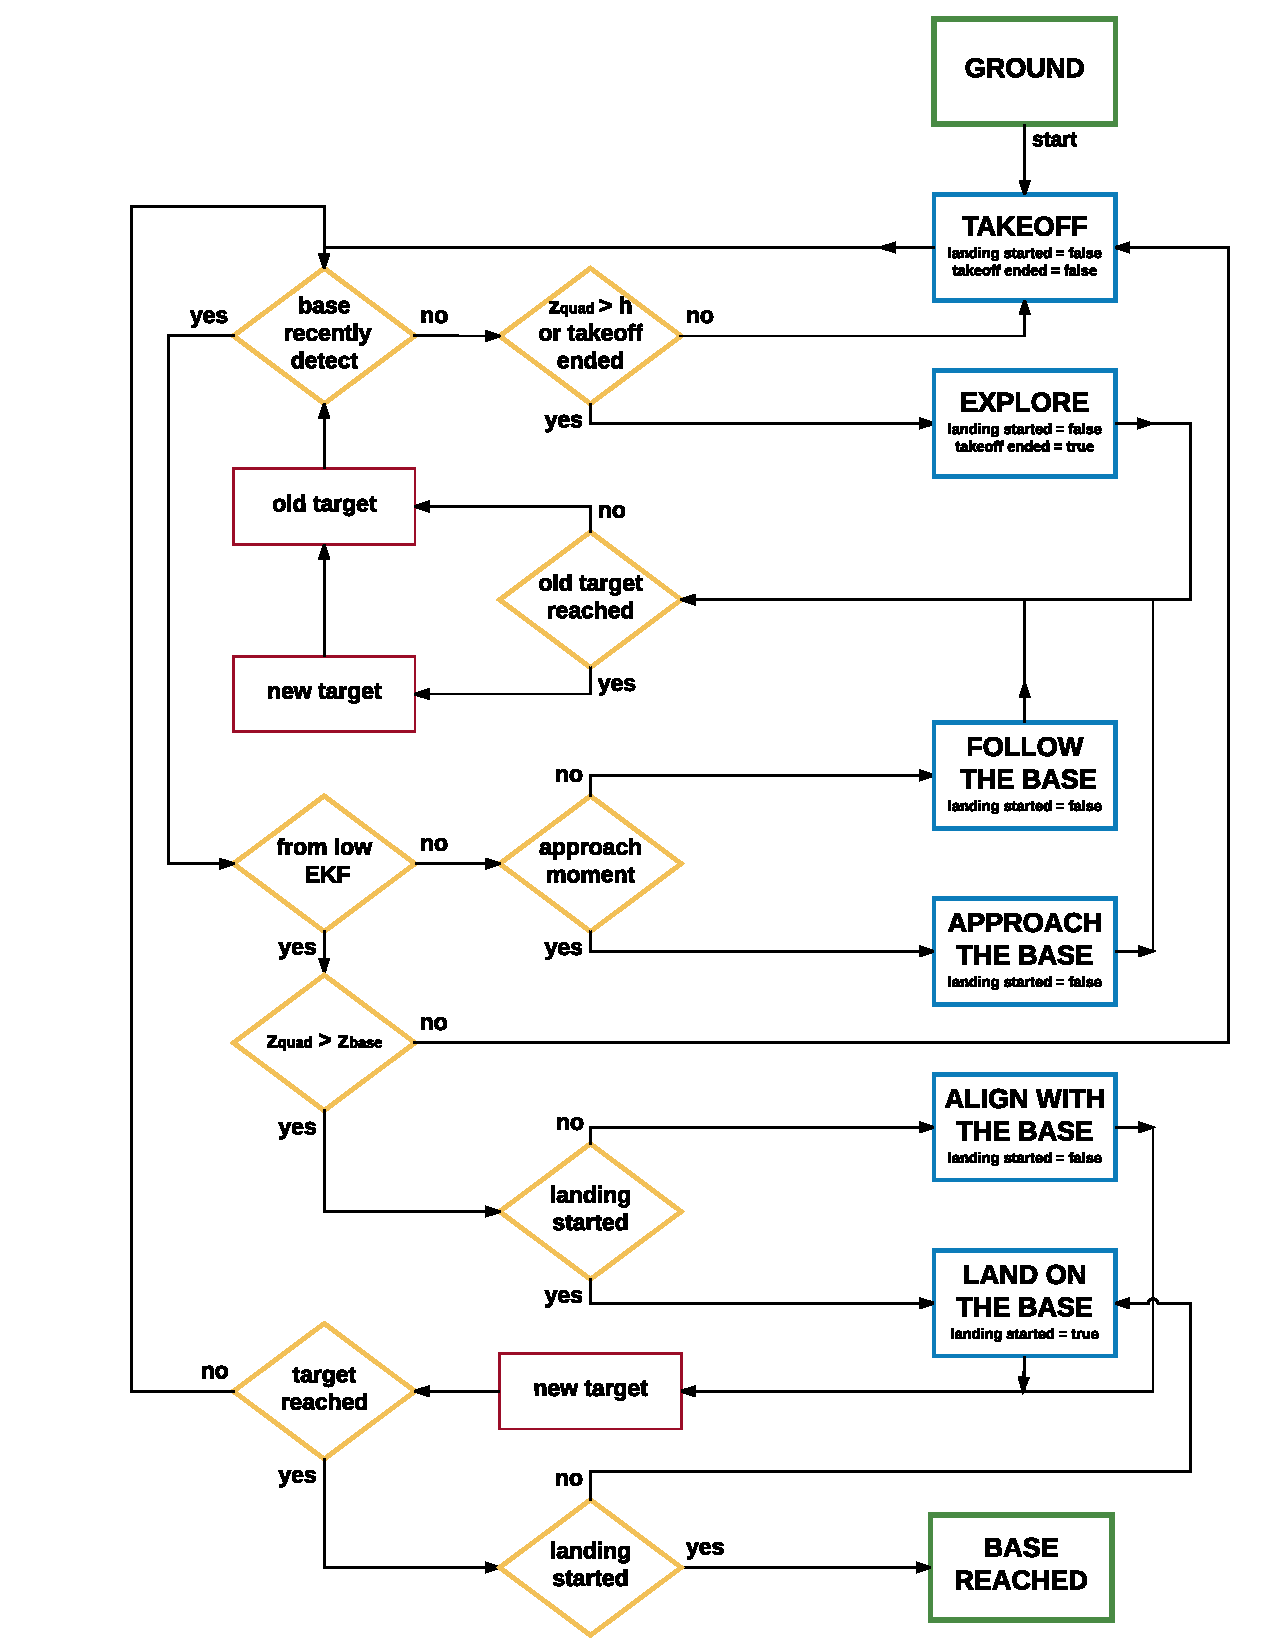
\includegraphics[width=1\textwidth]{img/state_machine.pdf}
    \caption{State machine flow chart}
    \label{fig:area_exploration_state_machine}
\end{figure}

It consists in 5 main parts in each of which the MAV has to complete a particular task in order to proceed with the successive stage. The task is defined by a precise final state that the quad must reach, and this final condition is considered reached when the position of the quad is inside a sphere of radius $\rho_{reached}$ and center the final state.\\

In the following sections we will describe in detail all these stages and explain the computation that we perform in order to decide where the UAV must go and when a particular stage is considered concluded.


\section{Takeoff and searching for the base}
In this stage the quadrotor starts from a static position near to the ground and has to explore a given area from high altitude until the platform is found.\\

At the beginning the quad is hovering close to the ground, then a vertical takeoff is performed until it reaches a given altitude $h$ (this vertical maneuver is performed anytime in which the pipeline fails and we have to restart the state machine).\\
Now given the area that must be explored to find the target (in our case it will be the arena in which the platform can move \ref{fig:arenachallenge}), we calculate a list of way-points the UAV must reach in order to span the whole surface.\\
While the quadrotor is moving the camera is collecting information from a large section of the space and the searching task of the target can be performed faster.\\
There are many ways to sample the way-points to explore the area, in our case we try to maximize the probability to find the moving platform so we are moving from one side to the other, along the main axis of the 8 shape path.\\

As soon as the moving platform is found the state machine proceeds with the next stage.

\section{Following the base}
In this stage the quadrotor has to following the moving platform until the right moment for starting the real landing maneuvers is come.\\

The MAV is moving at high altitude, reaching the desire points given by the previous stage.  As soon as an estimation of the target odometry is available, the quad begins to follow the platform and perform some computations in order to complete the task of this stage.

\subsection{Understand type of movement}
From the challenge description \ref{fig:arenachallenge} we know that the car is moving in a shape composed by straight lines and circumference sectors. We need to understand, at a given time, in which part the platform is: this information is important in order to calculate properly where the platform will be in $t$ seconds and because we want to proceed with the following phases, and perform the landing maneuver, when the platform is going straight.\\

To understand the trajectory of the moving base, we collect all the estimated positions of the base coming from the previous module \ref{chap:base_tracking}, and we perform a linear regression on the last $n$ estimations: the platform is moving in a straight line if the linear regression is a good approximation of the data trends otherwise it driving in a curve.\\

We have a series of $n$ points, each of these is consider as a pair of coordinates $(x_i,y_i)$, and we are searching for he best-fit line that can describe the data as a linear function: 
\begin{align*}
y = mx + q
\end{align*}
In our case there are no real dependent and independent variables so we perform the following analysis considering before the coordinates $y_i$ as dependent, then solve the dual problem with $x_i$, and finally peaking the best of this two fits. \\
We want find the best best parameters $m$ and $q$, and to do so we need to have some measure of quality to optimize. Unless all our $n$ points are already in a perfect line there will be an error between the value predicted by the line, and the observed dependent variable:
\begin{align}
e_i = y_i - (mx_i + q)
\label{theor_resid}
\end{align}

These differences are called residuals and what we want is to find the model that minimizes: 
\begin{align*}
\sum_{i=1}^{n}{e_i^2}
\end{align*}
The model we find is the Least Squares Fit of the data. \\ 
We define also the cumulative residual as: 
\begin{align*}
e_{tot} = \sqrt{\sum_{i=1}^{n}{e_i^2}}
\end{align*}

The parameters $m$ and $q$ of the model, are found where $e_{tot}^2$ is minimized:
\begin{align}
\begin{split}
\frac{e_{tot}^2}{\partial m} = 0\\
\frac{e_{tot}^2}{\partial q} = 0
\end{split}
\label{eq:mandq1}
\end{align}

It is easy to demonstrate that the solution of \ref{eq:mandq1} is:
\begin{align}
\begin{split}
m &= \ddfrac{n\sum_{i=1}^{n}{x_iy_i} - \sum_{i=1}^{n}{x_i}\sum_{i=1}^{n}{y_i}}{n\sum_{i=1}^{n}{x_i^2} -( \sum_{i=1}^{n}{x_i})^2} \\[10pt]
q &= \ddfrac{ \sum_{i=1}^{n}{y_i}}{n} - m\ddfrac{ \sum_{i=1}^{n}{x_i}}{n}
\end{split}
\label{eq:mandq}
\end{align}

The platform is moving in the straight line if the cumulative residual $e_{tot}$ is below a threshold $th_{line}$, while if the error is above $th_{curve}$ the base is traveling the circumference.\\

To have a good interpretation of the data it is important to decide the three parameters $n$, $t_{line}$, $t_{curve}$ correctly:
\begin{itemize}
\item The first parameter $n$ is the number of samples to consider when we perform the linear regression. We chose it in order to consider poses that are along a curve with length:
\begin{align}
l_{curve} = \frac{\rho_8\pi}{4} \label{eq:lengthcurve} 
\end{align}
We know the forward constant velocity of the car $v_{tan}$, so we can calculate the time in which the platform is performing this curve:
\begin{align}
t_{curve} = \frac{l_{curve}}{v_{tan}} \label{eq:timecurve} 
\end{align}

When we receive a pose at time $t_i$ we store it and we perform the linear regression with all the data stored from $[t_i-t_{curve},t_i]$.

\item The threshold parameters are calculating considering that each measure is corrupted by an additive Gaussian noise with 0 mean and $\sigma_e^2$ variance: 
\begin{align}
\tilde{y_i} = \mathcal{N}(y_i,\sigma_e^2) 
\end{align}
When we perform the linear regression on the measured data, the average residual square is 
\begin{align}
\begin{split}
<\tilde{e_i}^2> &= <(\tilde{y_i} - (mx_i + q))^2>  \\[5pt]
&= <\tilde{y_i}^2 - 2\tilde{y_i}(mx_i + q) + (mx_i + q)^2>  \\[5pt]
&= <\tilde{y_i}^2> - 2<\tilde{y_i}>(mx_i + q) + (mx_i + q)^2 \\[5pt]
&=  \sigma_e^2 + y_i^2  - 2y_i(mx_i + q) + (mx_i + q)^2  \\[5pt]
&=  \sigma_e^2 + e_i^2 
\end{split}
\end{align}

\begin{itemize}
\item when we perform the linear regression on linear data the theoretical data are distributed as:
\begin{align*}
\begin{cases}
x_i = x_i \\[10pt]
y_i = ax_i + b
\end{cases}
\end{align*} 
so the theoretical residual,, calculated using \ref{theor_resid}, is: 
\begin{align*}
e_i = ax_i + b - (mx_i + q)
\end{align*}
Of course when we try to calculate the model parameter $m$ and $q$ with \ref{eq:mandq}  the result will lead to:
 \begin{align}
\begin{split}
m &= a  \\[5pt]
q &= b
\end{split}
\label{eq:mandqcirum}
\end{align}
So, obviously, the theoretical residual squares is:
\begin{align*}
e_i^2  = 0
\end{align*} 
And the average residual squares on the measured data is:
\begin{align*}
<\tilde{e_i}^2>  = \sigma_e^2
\end{align*} 
The parameter $th_{line}$ is then:
\begin{align}
\begin{split}
th_{line} = \sqrt{\sum_{i=1}^{n}{\tilde{e_i}^2}} = \sqrt{\sum_{i=1}^{n}{\sigma_e^2}} = \sigma_e\sqrt{n}
\end{split}
\end{align}
\item When we perform the linear regression on data along a circumference arch with radius $\rho$ and angles $\theta_i \in [\theta_1,\theta_2]$ the theoretical data are distributed as:
\begin{align*}
\begin{cases}
x_i = \rho\cos{\theta_i}\\[10pt]
y_i = \rho\sin{\theta_i}
\end{cases}
\end{align*} 
so the theoretical residual, calculated using \ref{theor_resid}, is:
\begin{align*}
e_i = \rho\sin{\theta_i} - (m\rho\cos{\theta_i} + q)
\end{align*}
To find $m$ and $q$ we use equation \ref{eq:mandq}, but we want a general approximation of these values. To do so, we have  to consider all the sums in the equations as integrals, using the relation:
\begin{align}
\begin{split}
\lim_{n \to \infty} { \frac{b-a}{n} \sum_{i=0}^{n}{f(x_i)}} &=   \int_a^b{f(x )\mathrm  {d}x} \\[10pt]
 \sum_{i=0}^{n}{f(x_i)} &\simeq \frac{n}{b-a} \int_a^b{f(x )\mathrm  {d}x}
\end{split}
\label{eq:integralsandsums}
\end{align} 

So now if we calculate this approximation for our values we have:
\begin{align}
\begin{split}
\sum_{i=1}^{n}{x_iy_i} &= \sum_{i=1}^{n}{\rho^2\cos{\theta_i}\sin{\theta_i}}   \\
& \simeq  \frac{n}{\theta_2 - \theta_1}  \rho^2 \int_{\theta_1}^{\theta_2}{\cos{x}\sin{x} \mathrm  {d}x} \\
&=  \frac{n}{\theta_2 - \theta_1}  \frac{ \rho^2}{2} \Big[-\cos^2{x} \Big]_{\theta_2}^{\theta_2} \\[10pt]
 \sum_{i=1}^{n}{x_i} &= \sum_{i=1}^{n}{\rho\cos{\theta_i}} \\
&\simeq  \frac{n}{\theta_2 - \theta_1}  \rho \int_{\theta_1}^{\theta_2}{\cos{x}\mathrm  {d}x} \\
&= \frac{n}{\theta_2 - \theta_1}  \rho \Big[\sin{x} \Big]_{\theta_2}^{\theta_2}\\[10pt]
 \sum_{i=1}^{n}{y_i} &= \sum_{i=1}^{n}{\rho\sin{\theta_i}} \\
& \simeq  \frac{n}{\theta_2 - \theta_1}  \rho \int_{\theta_1}^{\theta_2}{\sin{x}\mathrm  {d}x} \\
&= \frac{n}{\theta_2 - \theta_1}  \rho \Big[-\cos{x} \Big]_{\theta_2}^{\theta_2}\\[10pt]
 \sum_{i=1}^{n}{x_i^2} &= \sum_{i=1}^{n}{\rho^2\cos^2{\theta_i}} \\
& \simeq  \frac{n}{\theta_2 - \theta_1}  \rho^2 \int_{\theta_1}^{\theta_2}{\cos^2{x}\mathrm  {d}x} \\
&=  \frac{n}{\theta_2 - \theta_1}  \frac{ \rho^2}{2} \Big[ x+\cos{x} \sin{x}\Big]_{\theta_2}^{\theta_2}
\end{split}
\label{eq:mandqintegralsoncircum}
\end{align}

In our case we consider pieces of curve with length $l_{curve}$ (defined in \ref{eq:lengthcurve}), that corresponds to a circumference arch with:
\begin{align}
\rho = \rho_8  \ \ \ \ \ \ \ \ \ \ \ \ \ 
\theta_i \in \Big[0,\frac{\pi}{4}\Big]
\label{eq:valuessircum}
\end{align}

We can now calculate the approximate values of $m$ and $q$ using \ref{eq:mandq} \ref{eq:mandqintegralsoncircum} \ref{eq:valuessircum}:
\begin{align}
\begin{split}
m &= \ddfrac{n\rho_8^2\frac{n}{\pi} - \rho_8\frac{n2\sqrt{2}}{\pi} \rho_8\frac{n2(2-\sqrt{2})}{\pi} }{n\frac{n\rho_8^2(2+\pi)}{2\pi} -(\rho_8\frac{n2\sqrt{2}}{\pi})^2}\\
 &= \ddfrac{2\pi - 16\sqrt{2} + 16}{\pi^2 + 2\pi - 16}  \\[10pt]
q &= \ddfrac{ \rho_8\ddfrac{n2(2-\sqrt{2})}{\pi} }{n} - m\ddfrac{ \rho_8\frac{n2\sqrt{2}}{\pi}}{n}\\
 &= \rho_8 \ddfrac{4-2\sqrt{2}(m+1)}{\pi} = \rho_8\bar{q} 
\end{split}
\label{eq:mandqcirum}
\end{align}
Now we should calculate the theoretical residual square $e_i^2$, but in this case we can compute the algebraic average residual square $<e_i^2>$, using again the approximations \ref{eq:mandqintegralsoncircum}, the values calculate in \ref{eq:mandqcirum}, and averaging over the $n$ samples we consider:
\begin{align}
\begin{split}
<e_i^2> &=  \frac{1}{n}\sum_{i = 1}^{n}{\Big(\rho_8\sin{\theta_i} - (m\rho_8\cos{\theta_i} + q)\Big)^2}\\
%&= \frac{1}{n}\sum_{i = 1}^{n}{\rho_8^2\sin^2{\theta_i} - 2\rho_8\sin{\theta_i}(m\rho_8\cos{\theta_i} + q) + (m\rho_8\cos{\theta_i} + q)^2}\\
& =  \frac{1}{n}\sum_{i = 1}^{n} \rho_8^2 \xi = \rho_8^2 \xi 
\end{split}
\end{align}
In particular with $\theta$ having values like in \ref{eq:valuessircum} we lead with:
\begin{align}
\xi &= \frac{\pi - 2 + m^2(\pi+2) + 2\pi\bar{q}^2 - 4m -8\bar{q}(2-\sqrt{2}+ m\sqrt{2})}{2\pi}
\end{align}
Finally we calculate 
\begin{align*} 
<\tilde{e_i}^2>  = <e_i^2> + \sigma_e^2 = \rho^2 \xi  + \sigma_e^2 
\end{align*} 
The parameter $th_{curve}$ is then:
\begin{align}
\begin{split}
th_{curve} = \sqrt{\sum_{i=1}^{n}{\tilde{e_i}^2}} = \sqrt{\sum_{i=1}^{n}{\rho^2 \xi  + \sigma_e^2}} = \sqrt{n}(\sigma_e + \rho\sqrt{\xi})
\end{split}
\end{align}
\end{itemize}
\end{itemize}

The figure \ref{fig:error_regression} shows the typical evolution of the total residual during this first stage: the different phases of linear and circular movement can be detect in the graph. Furthermore the point of regime change can be seen both in figure \ref{fig:error_regression}  and in the map \ref{fig:error_regression_map} in which also all the estimate positions of the base are plotted.

\begin{figure}[!htbp]
    \centering
    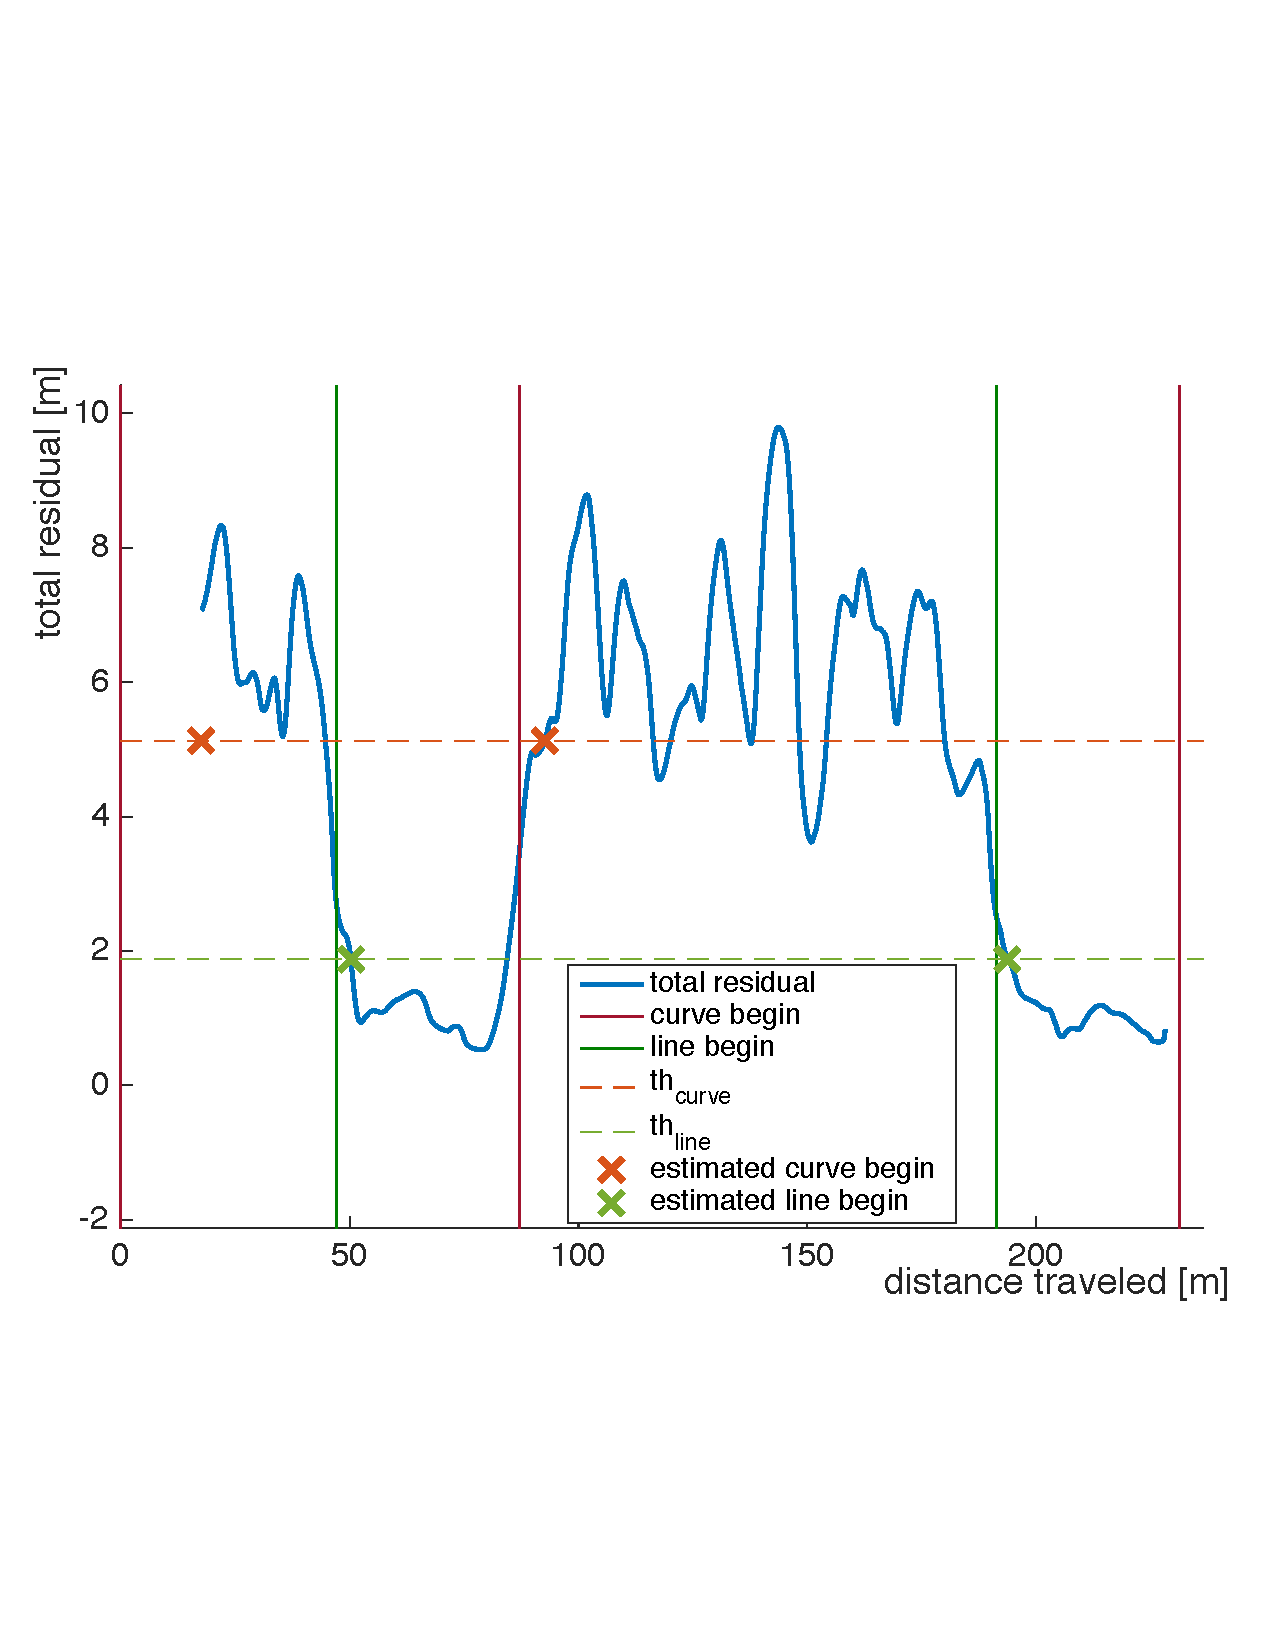
\includegraphics[width=0.9\textwidth, height=0.5\textwidth]{img/following_platform_for_long_position_base_error.pdf}
    \caption{Evolution of the total residual during this first phase (in blue). The vertical lines are the real moments in which the car changes movement types: green a linear phase starts, red a circular phase begins. The horizontal lines are the thresholds for the detection of the two different regimes. The cross are the moment in which the algorithm understands the change.}
    \label{fig:error_regression}
\end{figure}
\begin{figure}[!htbp]
    \centering
    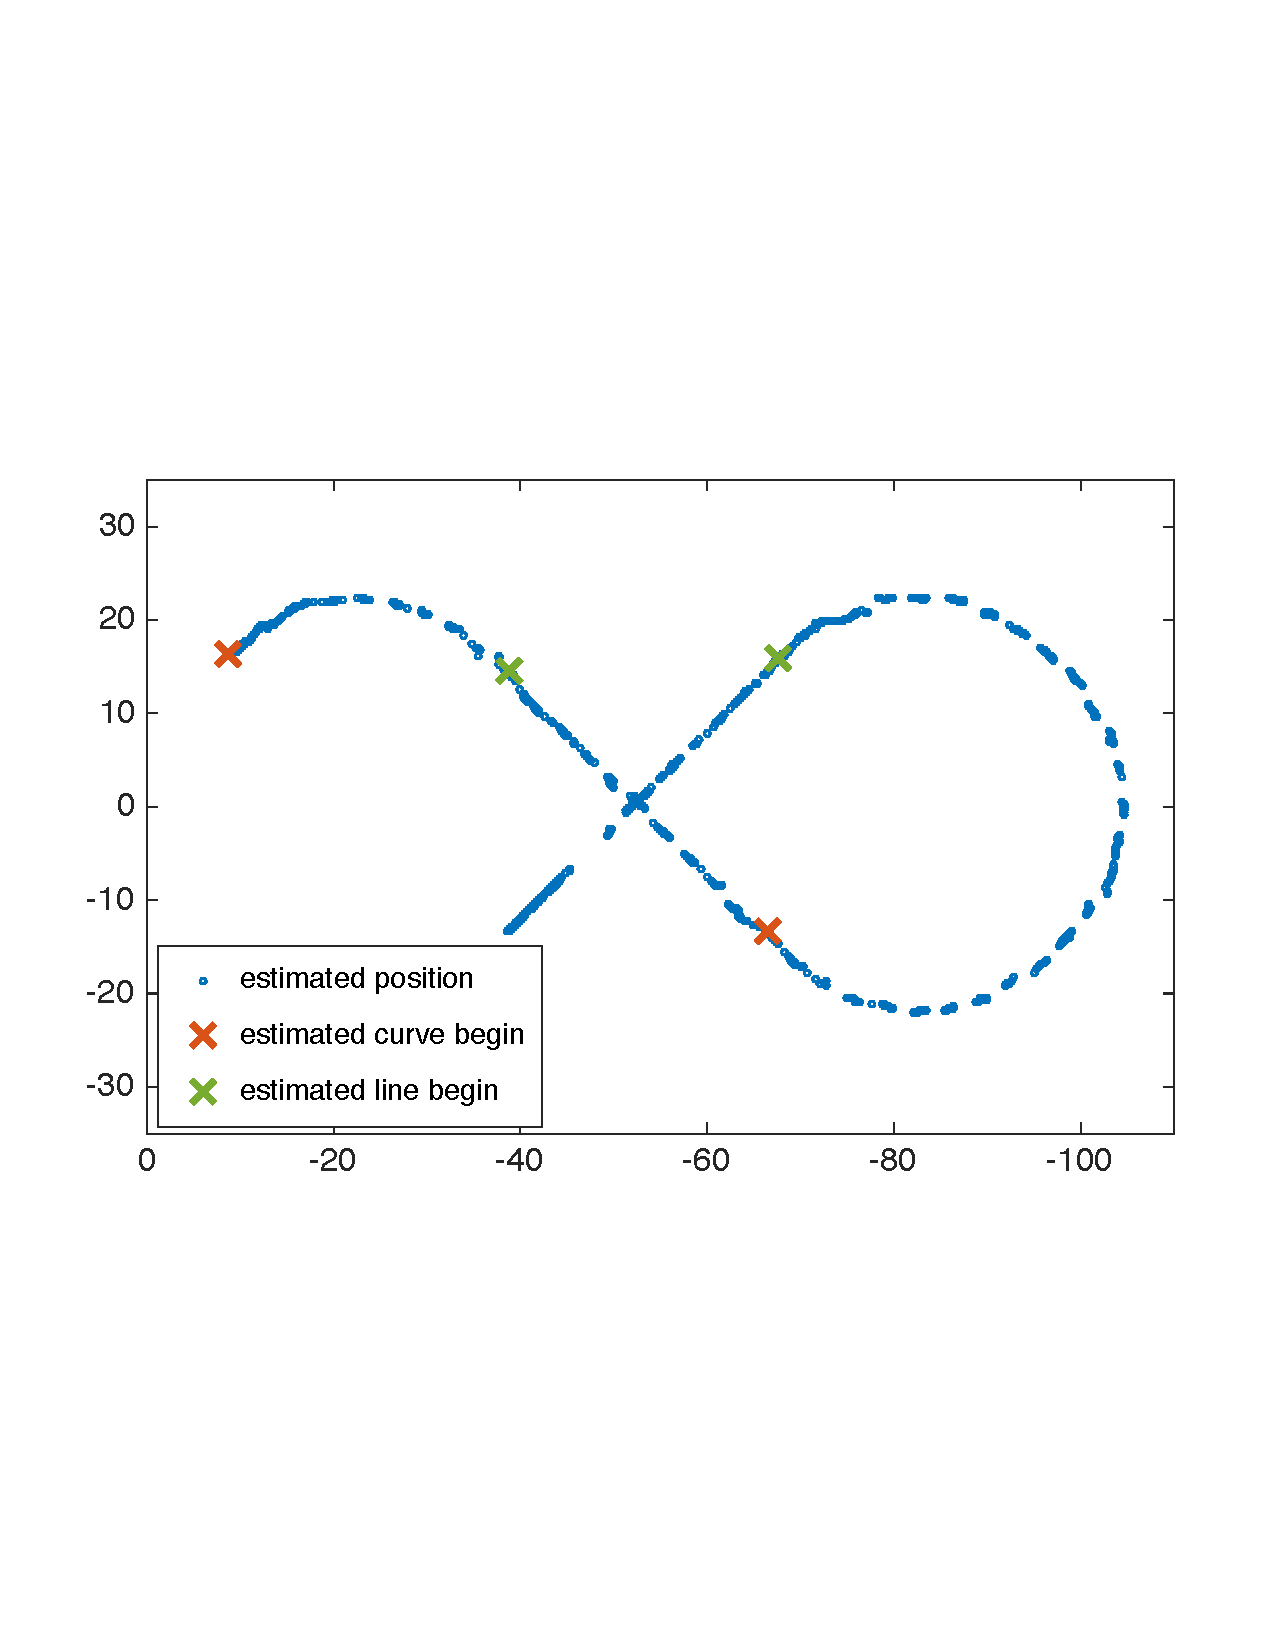
\includegraphics[width=0.8\textwidth]{img/following_platform_for_long_map_simple.pdf}
    \caption{Map of the estimated positions of the platform in blue. The crosses are the moments in which the algorithm understands the change. Red crosses from line to curve. Green crosses from curve to line.}
    \label{fig:error_regression_map}
\end{figure}

We can see from these graphs that with the method explained is possible to distinguish clearly the period of time in which the platform is traveling along a line or along a curve, and it is also finding the switching points with high accuracy.\\ 
The major drawback of this method is that it is necessary an amount of time equal to $t_{curve}$ to understand that the platform switched motion regime. \\
If  $th_{line}$ and  $th_{curve}$ will result too close it is always possible to consider a curve with longer length $l_{curve}$: this will increase much more the letter threshold w.r.t the former, but also will increase the time $t_{curve}$ to understand the type of movement.

\subsection{Calculate future position}
Now knowing the platform regime of movement at a specific time we can estimate correctly where it will be after $t_s$ seconds and proceed with the following stages when it starts a straight portion of the trajectory.\\
Thanks to the algorithm described before we can estimate that at the moment $t_0$ the car is at position $(x_0,y_0)$ with a direction angle of $\theta_0$ and forward velocity of $v_{tan}$, so at time $t_1 = t_0 + t_s$ seconds the car will be at position $(x_1,y_1)$ with an angle  $\theta_1$, and it has traveled  $v_{tan}t_s$.
\begin{itemize}
\item When no regime is found (at the begging) or when a line movement is detect, the predicted state is:
\begin{align}
\begin{cases}
x_1 &= x_0 + v_{tan}t_s\cos{\theta_0}\\[5pt]
y_1 &= y_0 + v_{tan}t_s\sin{\theta_0}\\[5pt]
\theta_1 &= \theta_0
\end{cases}
\label{eq:line_future_pose}
\end{align}
\item When a movement in the circumference is detected we have to perform some calculations in order to find the final state of the platform.\\ 
First of all we use the relation 
\begin{align*}
l_{curve} = v_{tan}t_s = \rho_8|\beta_s|
\end{align*}
Where $\beta_s$ is the angle spanned by the platform in $t_s$ seconds:
\begin{align}
|\beta_{s}| &= \frac{v_{tan}t_s}{\rho_8}
 \label{eq:anglespanned}
\end{align}
The final angle will be:
 \begin{align}
 \theta_1 = \theta_0 + \beta_s
 \label{eq:anglefinal}
 \end{align}

Referring to figure \ref{fig:chord} we can calculate that the segment connecting $(x_0,y_0)$ and $(x_1,y_1)$ has:
\begin{itemize}
\item direction $\theta_{chord}$ found as bisection between 
 $\theta_0$ and $\theta_1$
 \begin{align}
 \theta_{chord} = \theta_0 + \frac{\theta_0 + \theta_1}{2} 
 \label{eq:anglechord}
 \end{align}
\item length $l_{chord}$, found with the chord theorem:
\begin{align}
 l_{chord} = 2\rho_8\sin{\frac{|\beta_s|}{2}}
  \label{eq:lengthchord}
 \end{align}
\end{itemize}
\begin{figure}[!htbp]
    \centering
    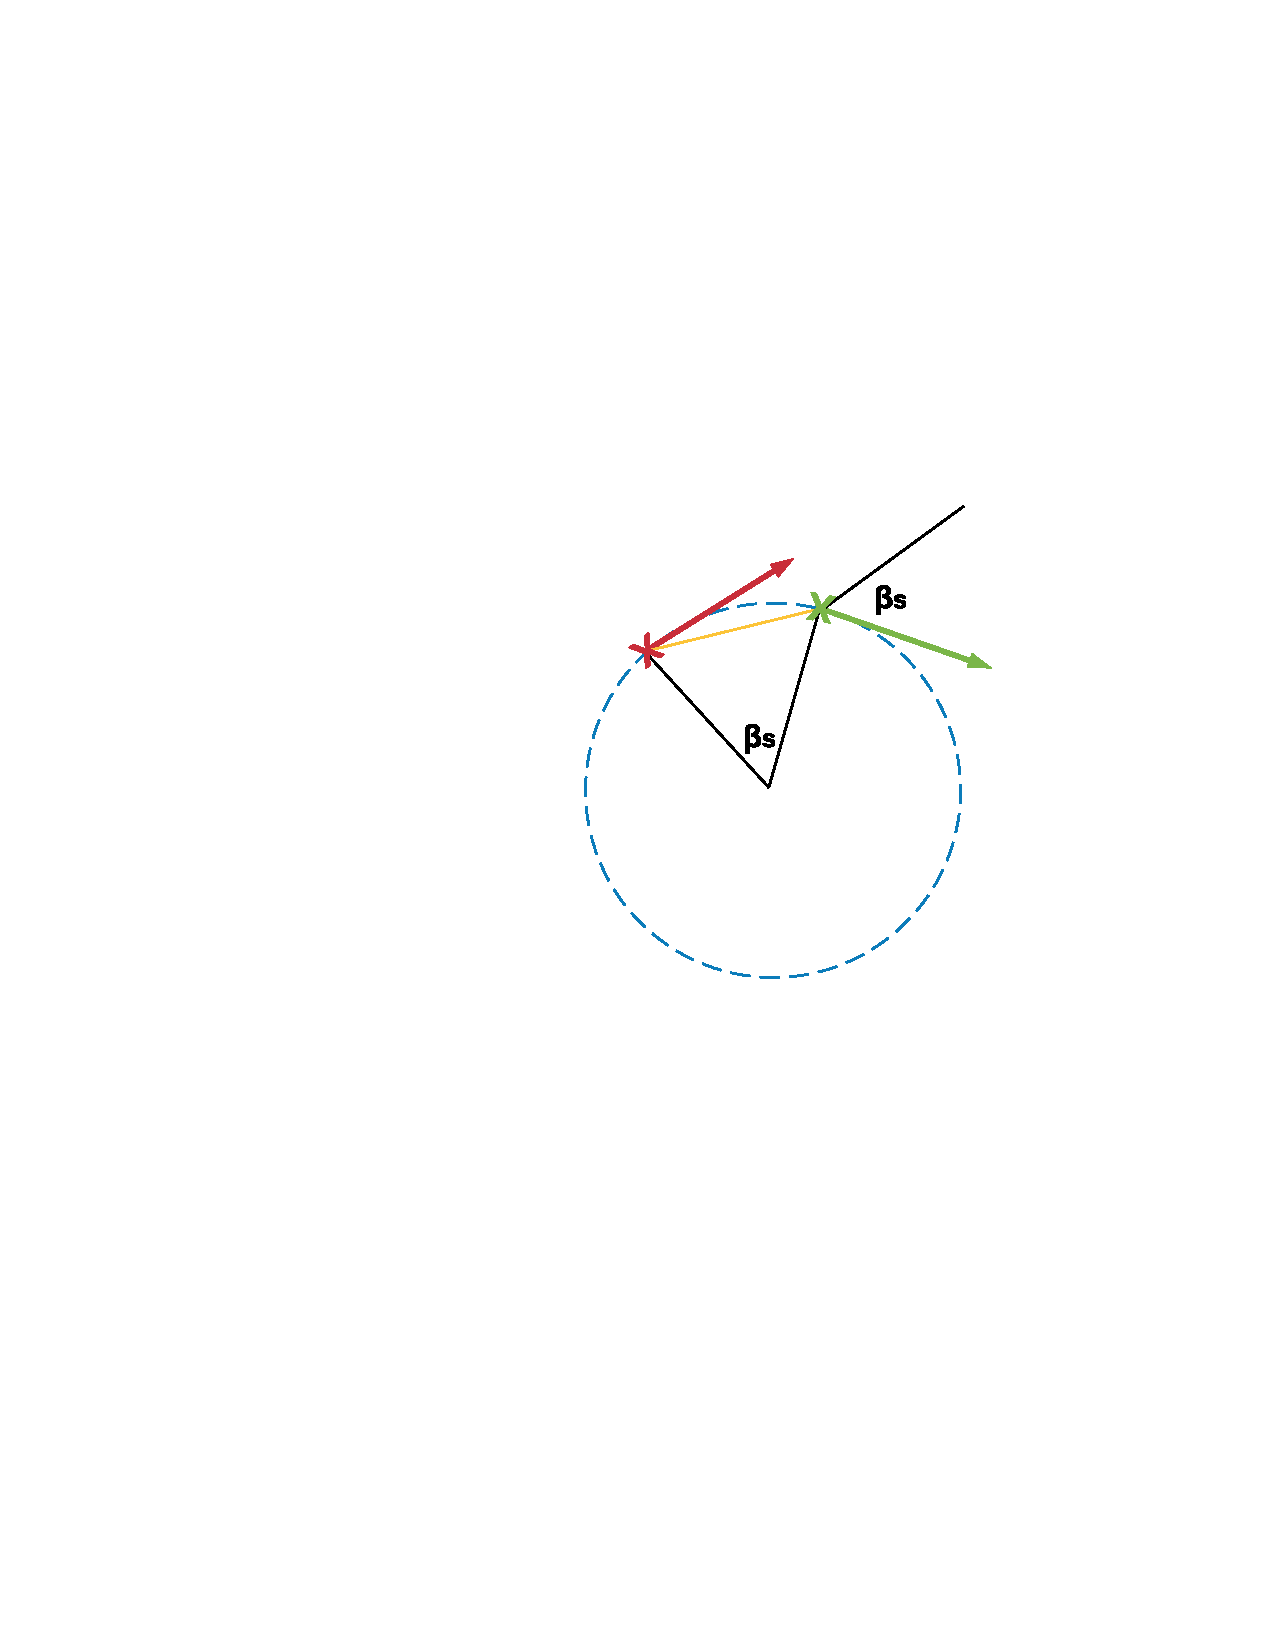
\includegraphics[width=0.5\textwidth]{img/chord.pdf}
    \caption{In red position of initial state at time $t_0$. In green final estimate state at time $t_1$. In yellow the chord between the two states with length $l_{chord}$ and orientation $\theta_{chord}$.}
    \label{fig:chord}
\end{figure}

Now we have all the elements to calculate the final point $(x_1,y_1)$, but in order to properly find it we have to resolve an other last problem: both $\beta_{s}$ and  $-\beta_{s}$ span a curve of length $v_{tan}t_s$, and due to the symmetry of our trajectory is impossible to know before which angle is the right one. \\
What we can do is calculate both the two possible final states using \ref{eq:anglespanned} \ref{eq:anglechord} \ref{eq:lengthchord}:
\begin{align*}
\begin{cases}
x_1^a &= x_0 + l_{chord}\cos{\Big(\theta_0 + \frac{|\beta_s|}{2}\Big) }\\[5pt]
y_1^a &= y_0 + l_{chord}\sin{\Big(\theta_0 + \frac{|\beta_s|}{2} \Big)}\\[5pt]
\theta_1^a &=  \theta_0 + |\beta_s|
\end{cases}
\end{align*}
\begin{align*}
\begin{cases}
x_1^b &= x_0 + l_{chord}\cos{\Big(\theta_0 - \frac{|\beta_s|}{2}\Big) }\\[5pt]
y_1^b &= y_0 + l_{chord}\sin{\Big(\theta_0 - \frac{|\beta_s|}{2}\Big) }\\[5pt]
\theta_1^b &=  \theta_0 - |\beta_s|
\end{cases}
\end{align*}

In order to understand which one is the correct state we can calculate the distance between the two possible final points and a point of the trajectory estimated at time $ t_{-\alpha} < t_0$. For sure the state with smaller distance will be the right final state, because the wrong one leads to a position further away.\\

The images  \ref{fig:sequence_find_next_position_circumference} summarize the passages we perform to find the right final state just explained.

\begin{figure}[!htbp]
  \centering
   \begin{subfigure}[b]{0.45\textwidth}
        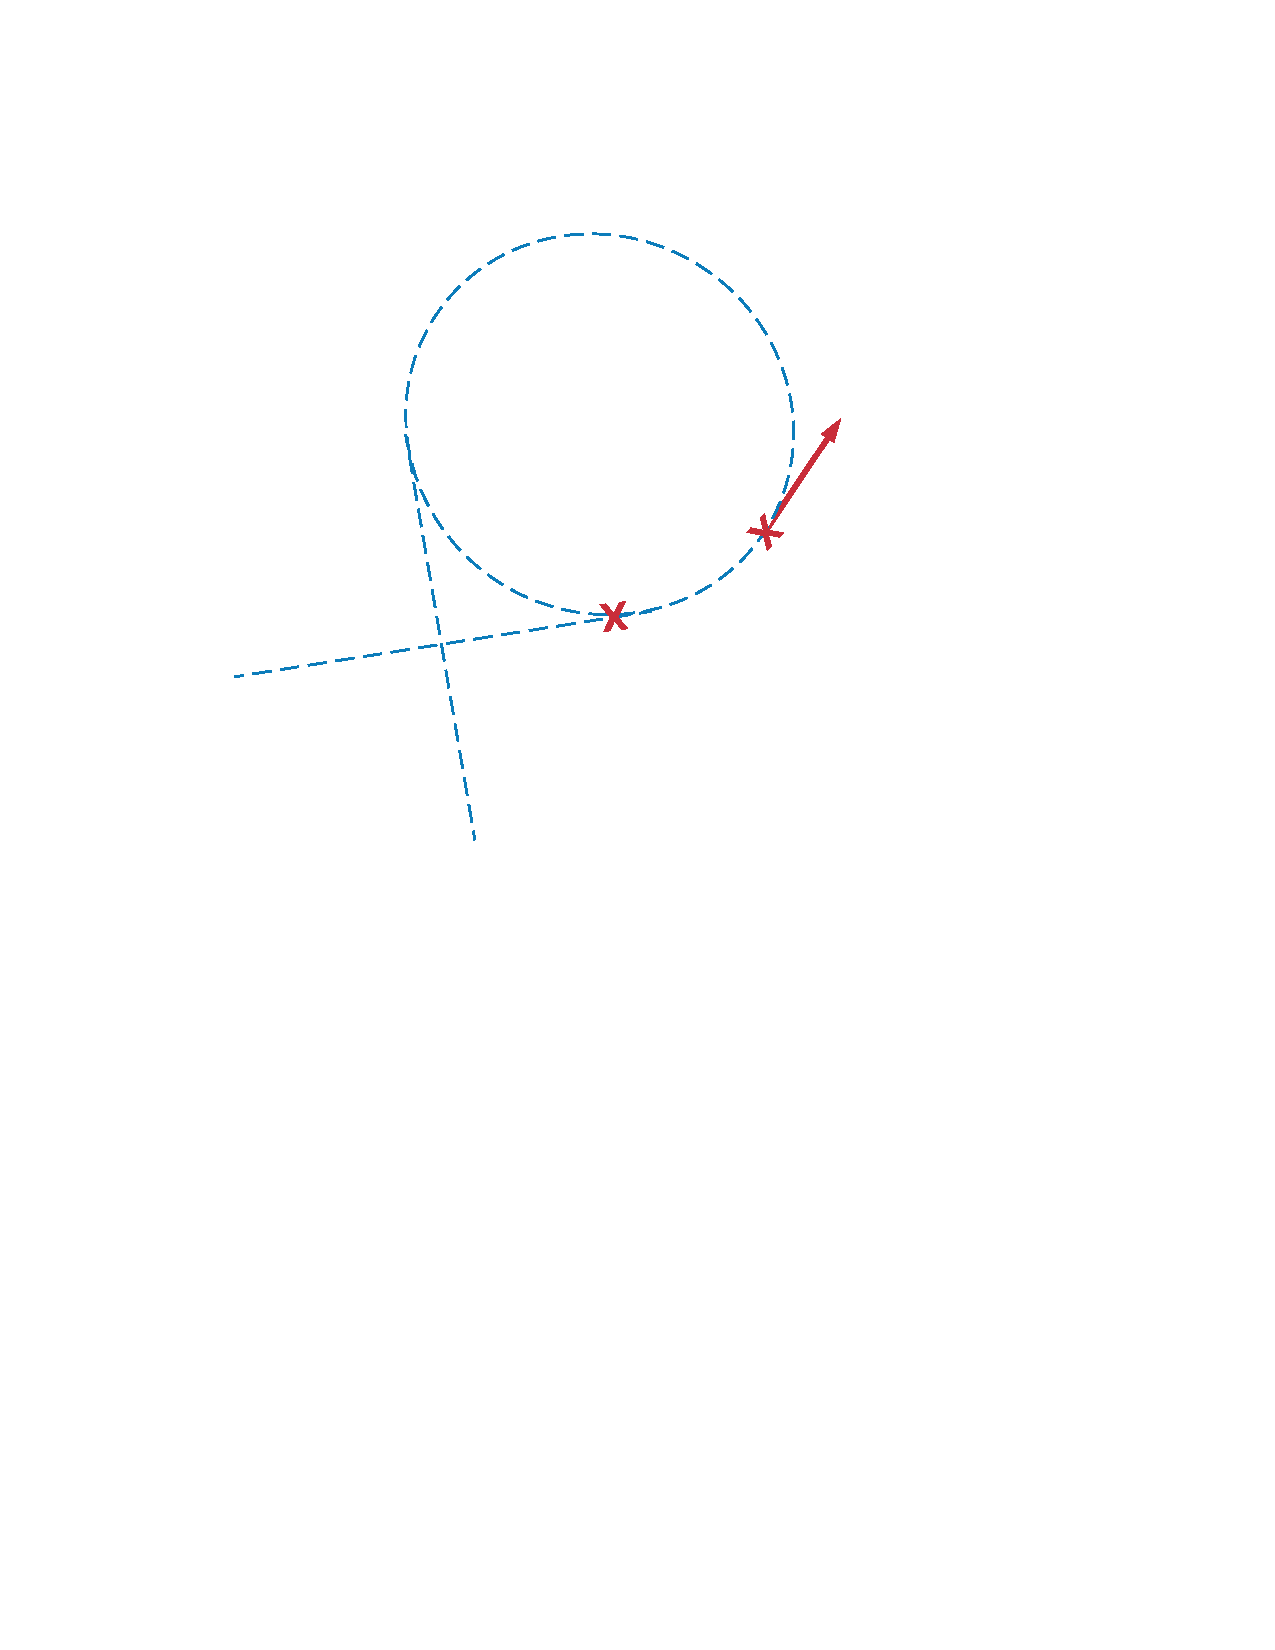
\includegraphics[width=\textwidth]{img/circular_movment1.pdf}
        \caption{Red cross with arrow: state a $t_0$. Red arrow: current velocity vector. Red cross: previous position a $t_{-\alpha}$.}
        \label{fig:one}
   \end{subfigure}\hfill
   \begin{subfigure}[b]{0.45\textwidth}
        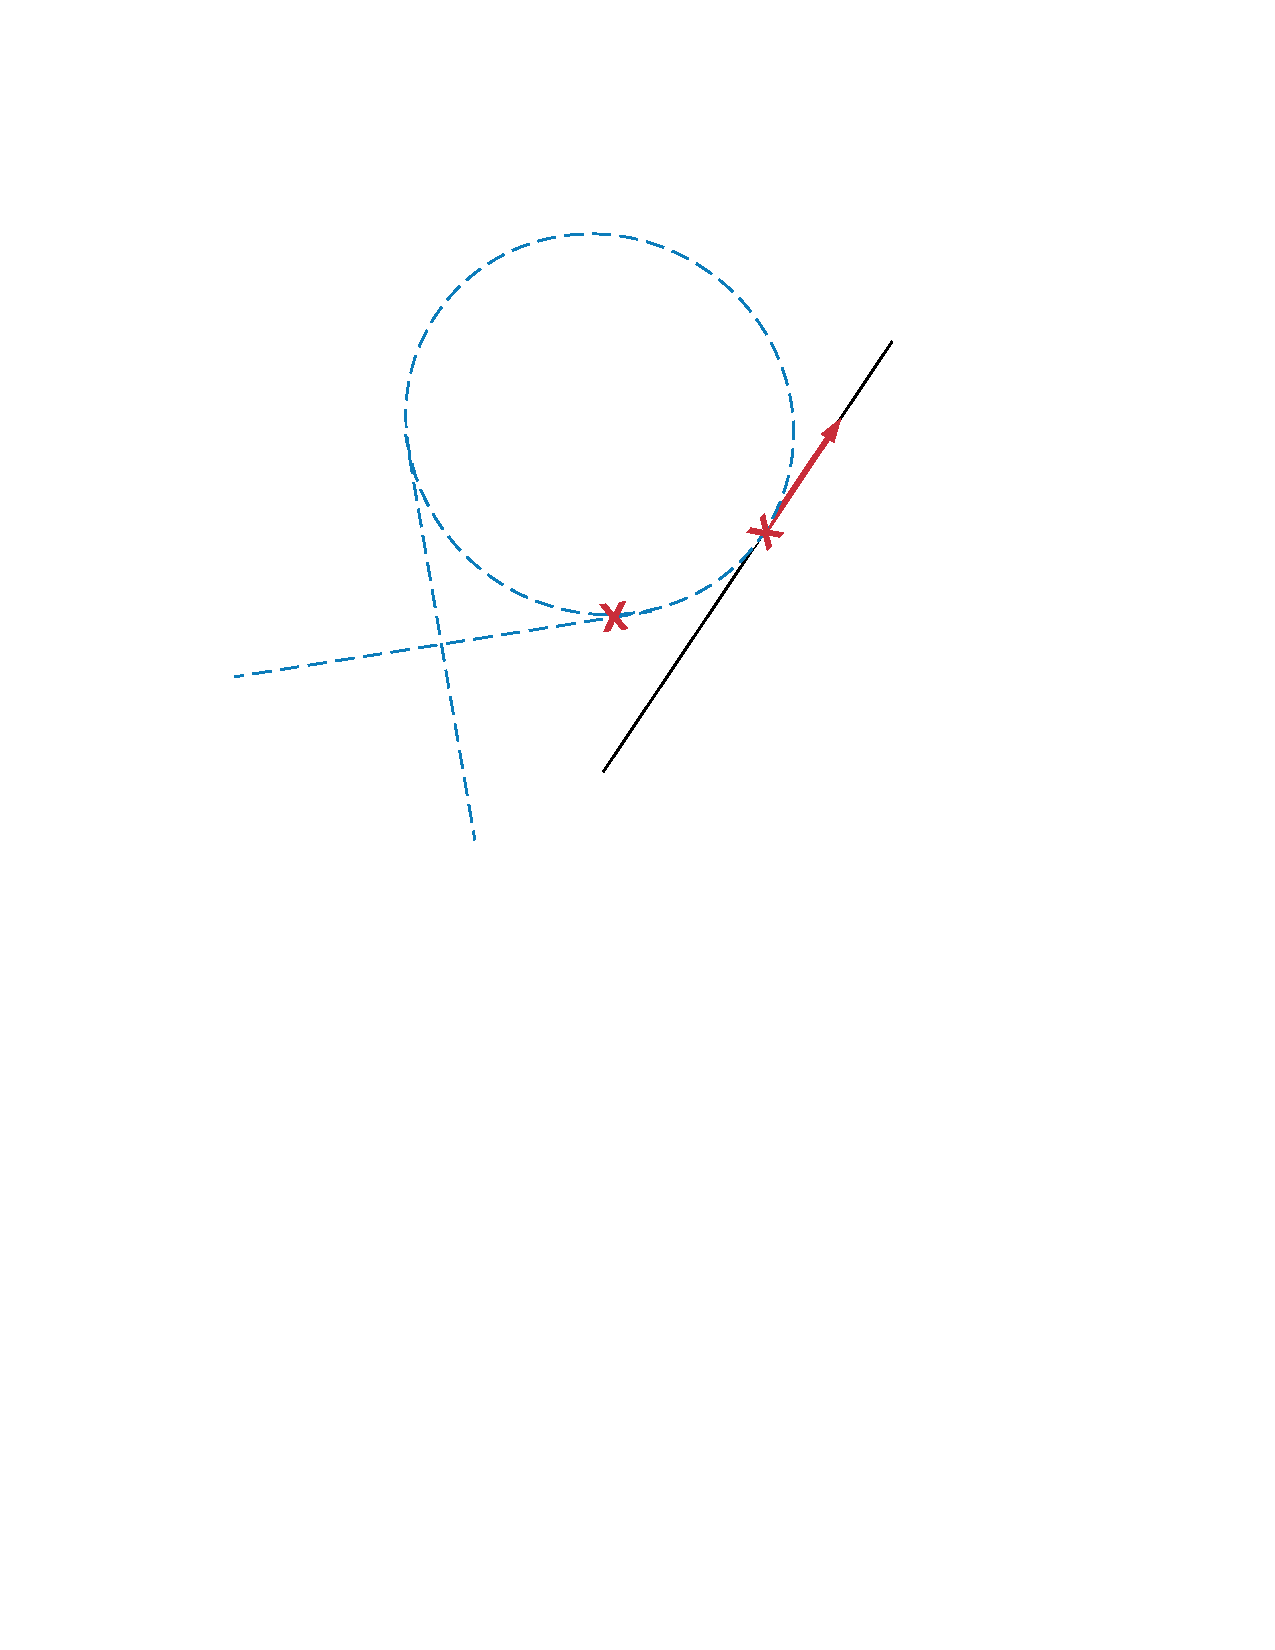
\includegraphics[width=\textwidth]{img/circular_movment2.pdf}
        \caption{Black line: direction of the velocity vector, with angle $\theta_0$. We have symmetry with respect to this axes.}
        \label{fig:two}
   \end{subfigure}
   
   \begin{subfigure}[b]{0.45\textwidth}
        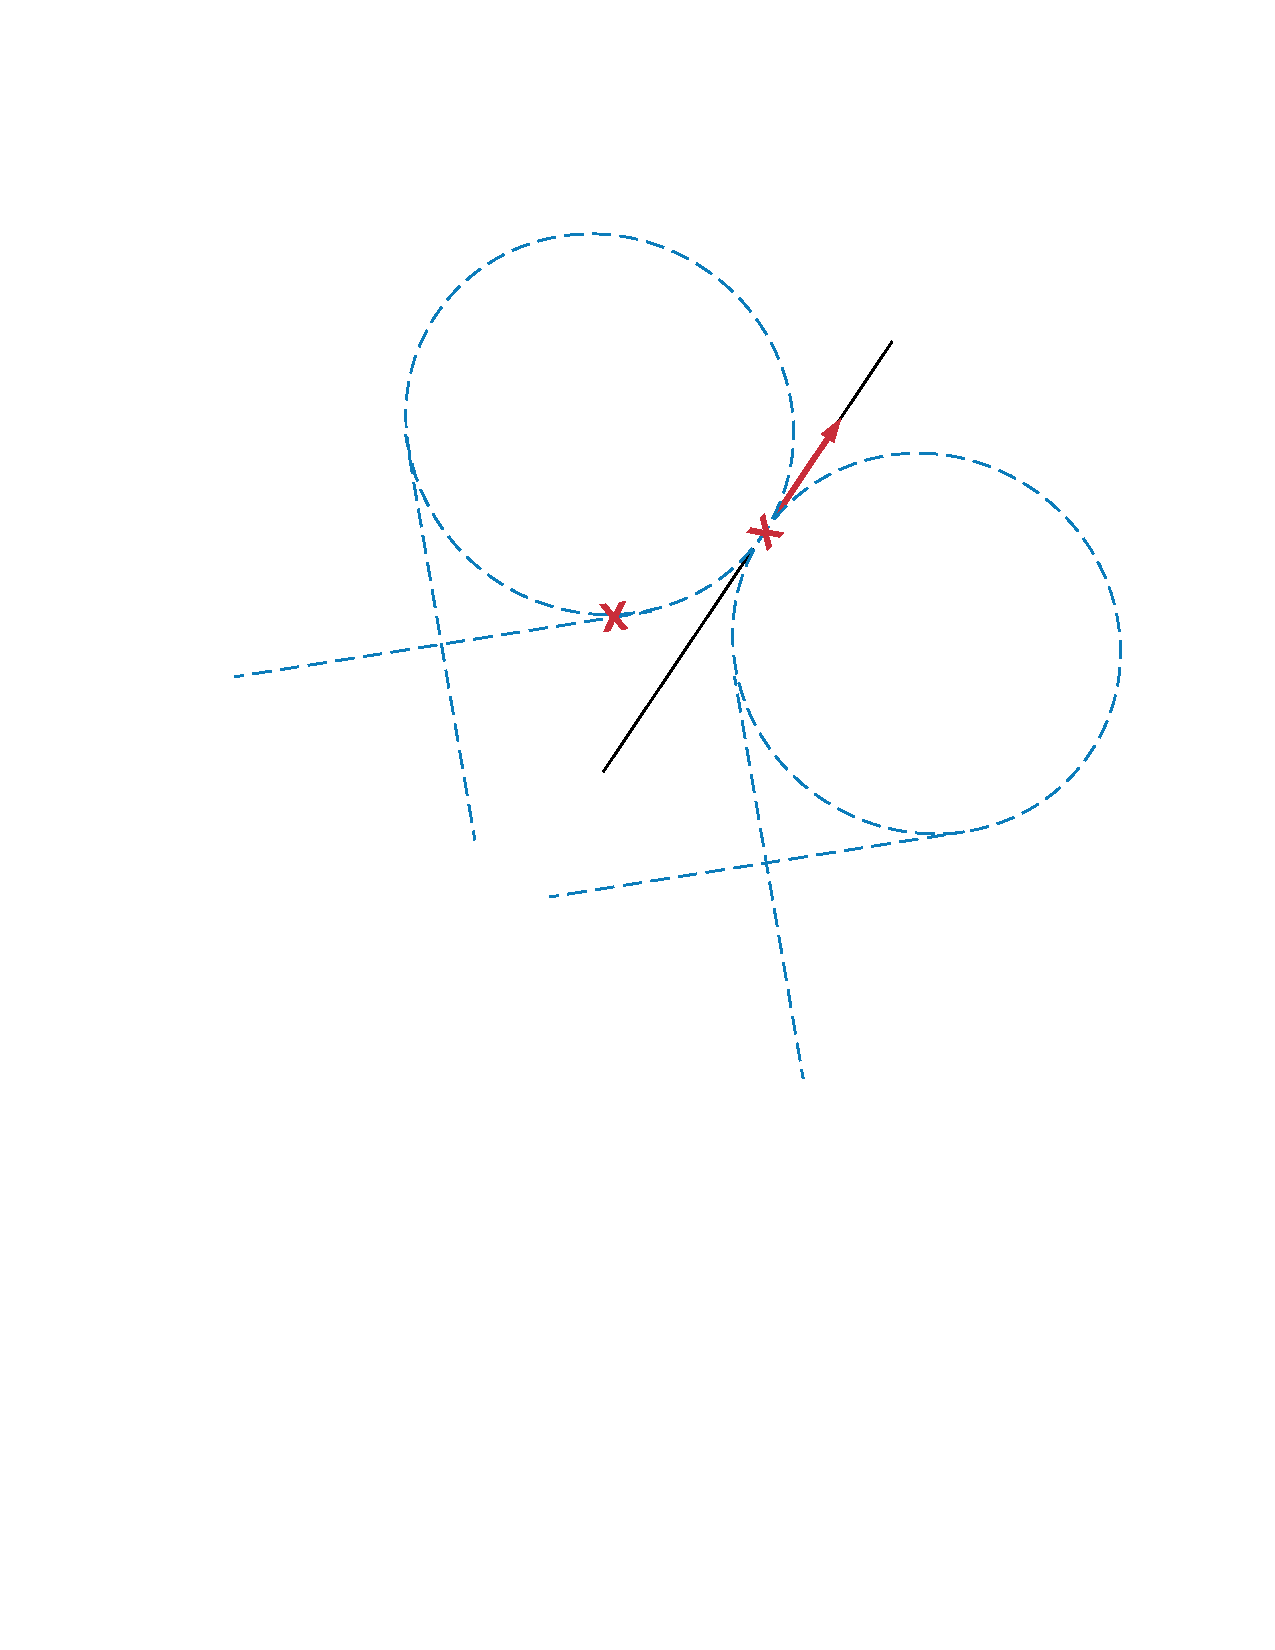
\includegraphics[width=\textwidth]{img/circular_movment3.pdf}
        \caption{Blue lines: real and symmetric path. We do not know which of the two trajectories is correct.}
        \label{fig:three}
   \end{subfigure}\hfill
    \begin{subfigure}[b]{0.45\textwidth}
        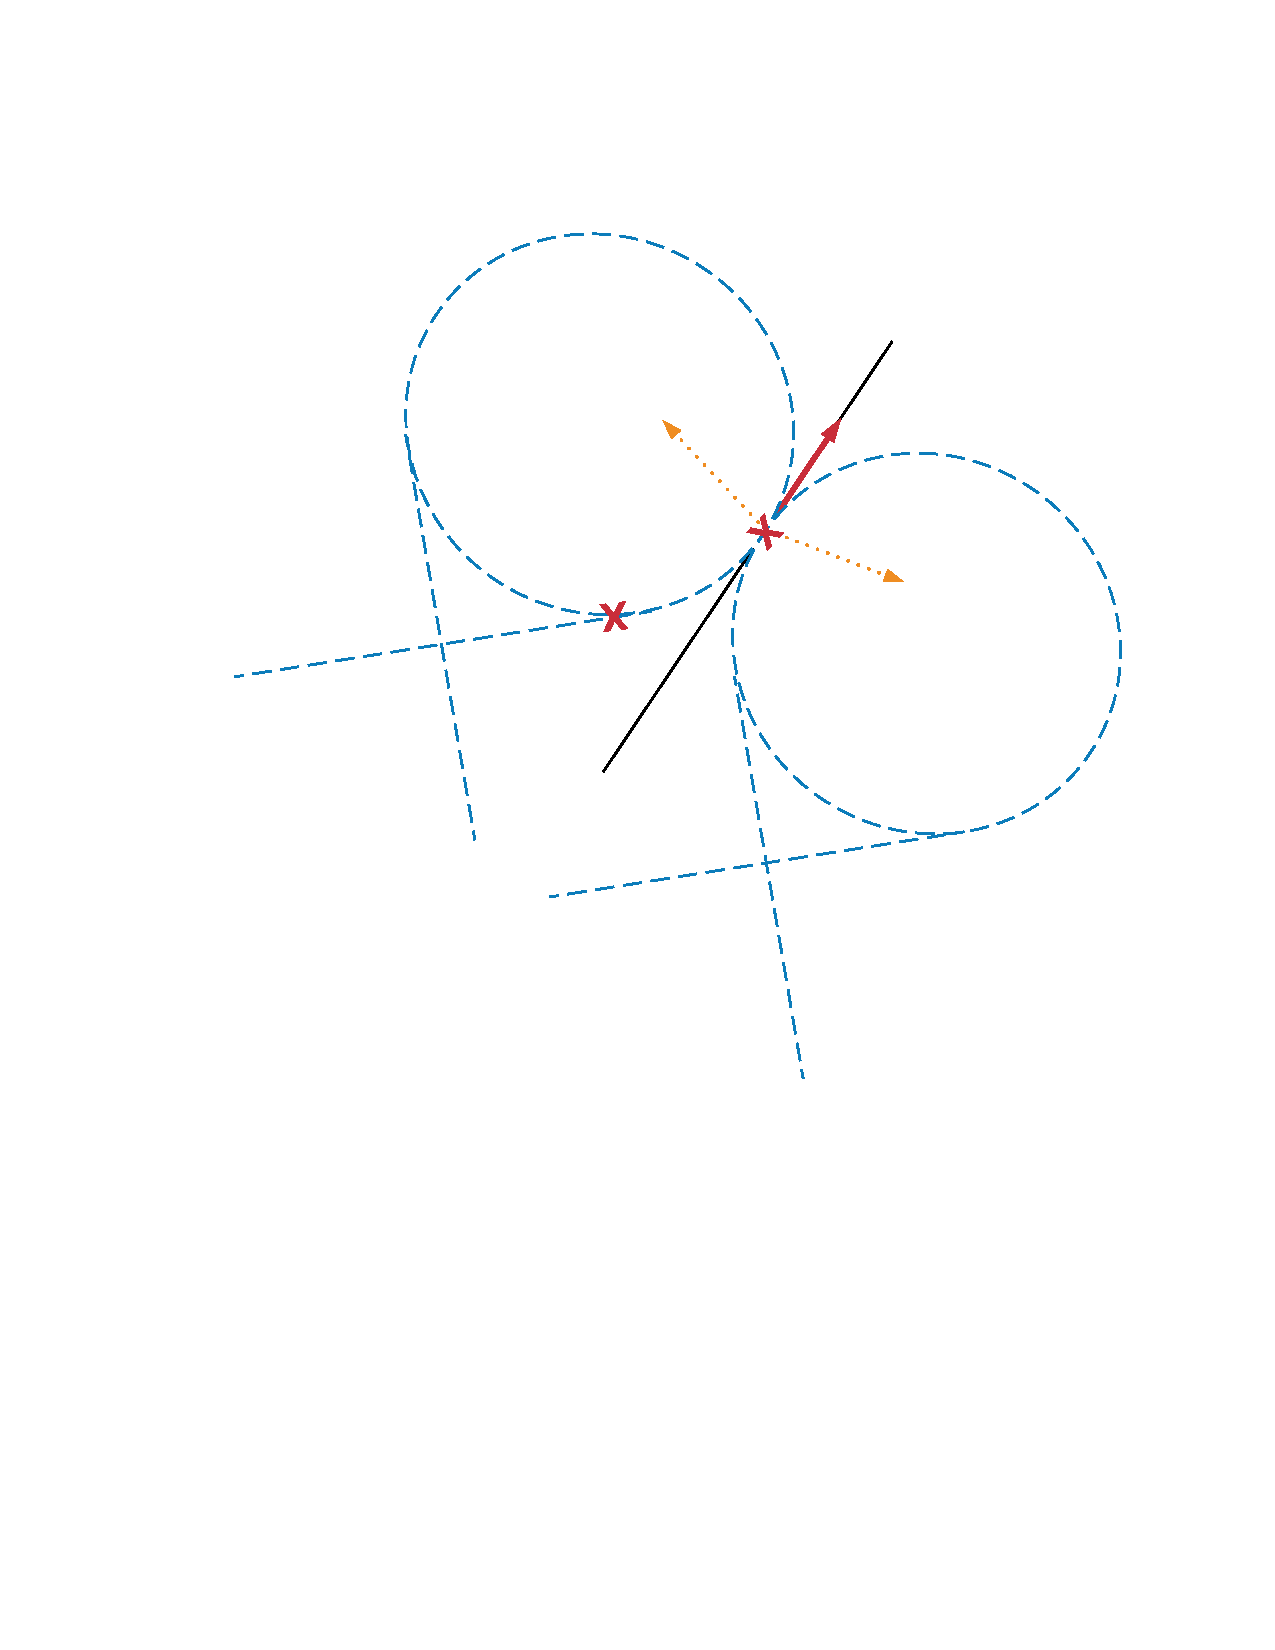
\includegraphics[width=\textwidth]{img/circular_movment4.pdf}
        \caption{Yellow arrows: estimated future angles $\theta_1^a$ and $\theta_1^b$ that the base will assume at time $t_1$.}
        \label{fig:four}
   \end{subfigure}
   
    \begin{subfigure}[b]{0.45\textwidth}
        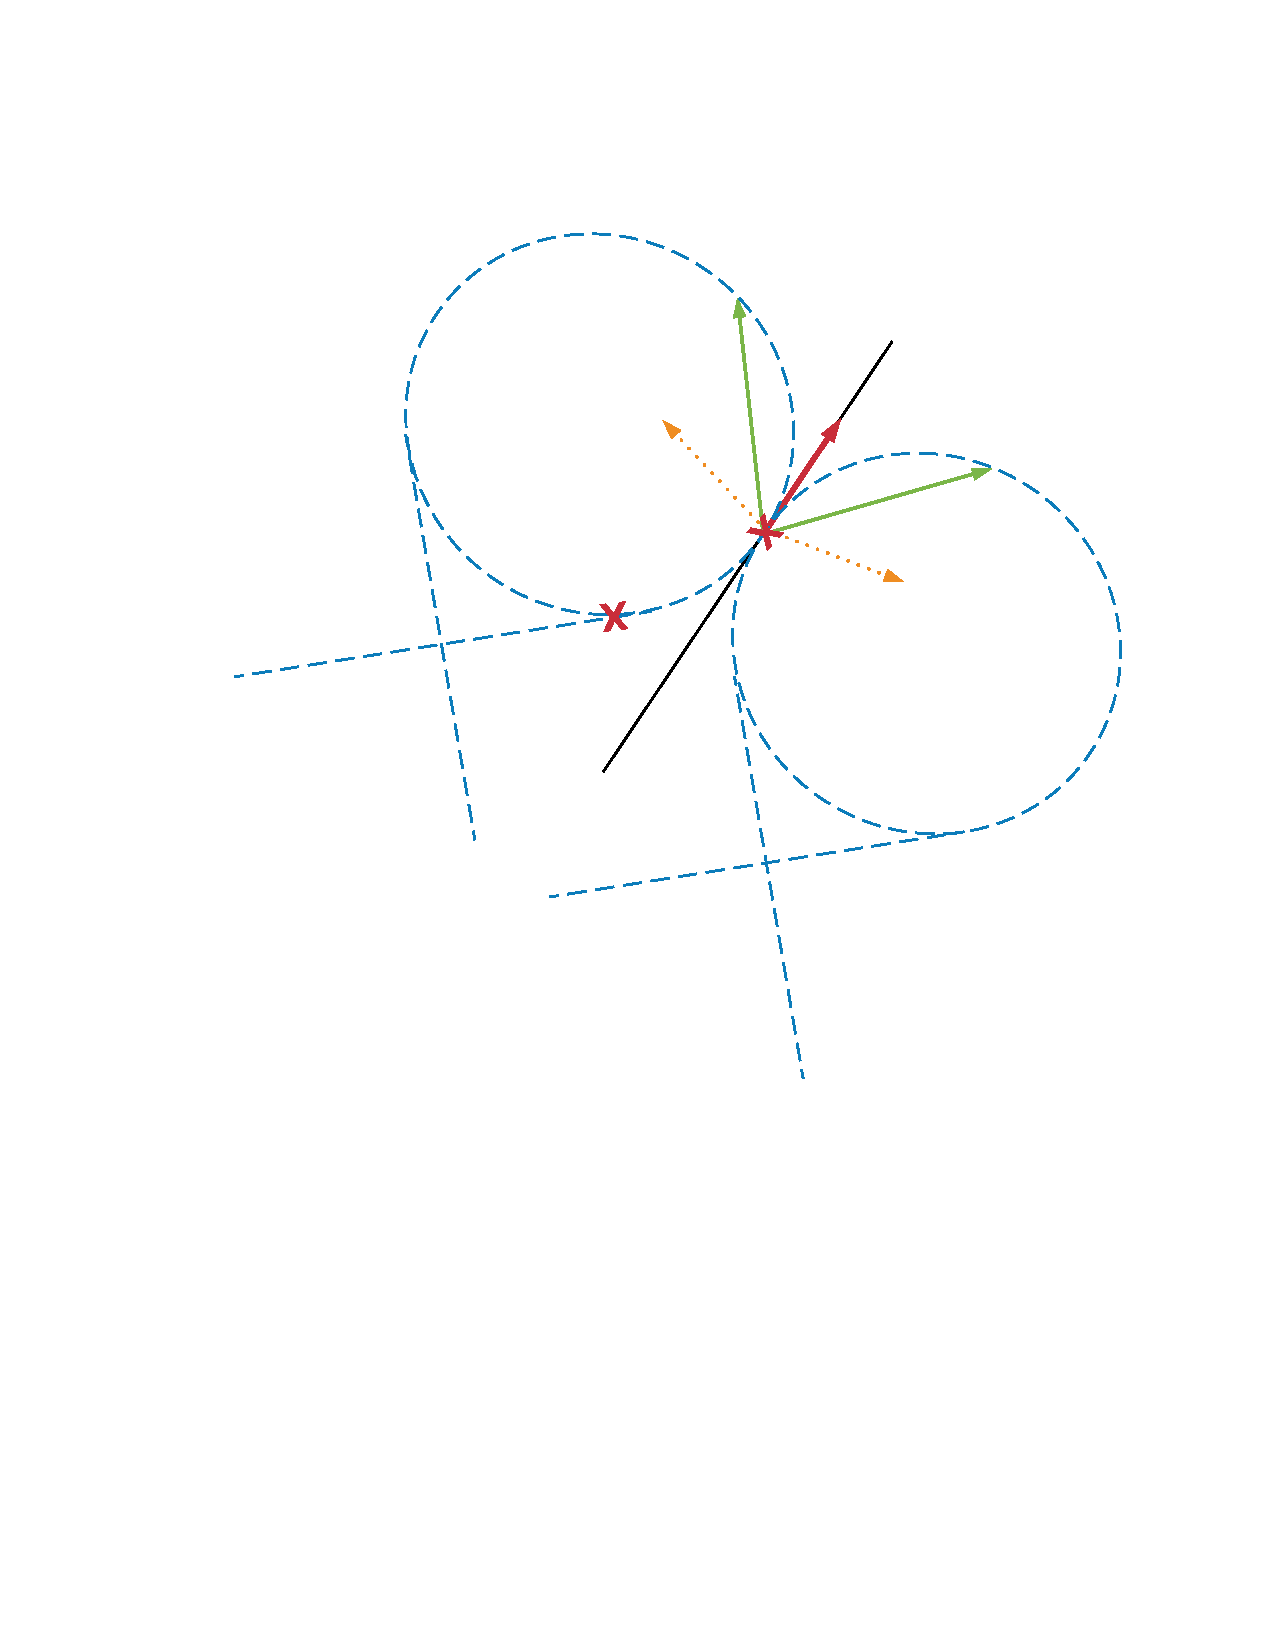
\includegraphics[width=\textwidth]{img/circular_movment5.pdf}
        \caption{Green arrows: segment from state at $t_0$ and possible states at $t_1$: with angles $\theta_{chord}^a$  and $\theta_{chord}^b$ and length $l_{chord}$ }
        \label{fig:five}
   \end{subfigure}\hfill
    \begin{subfigure}[b]{0.45\textwidth}
        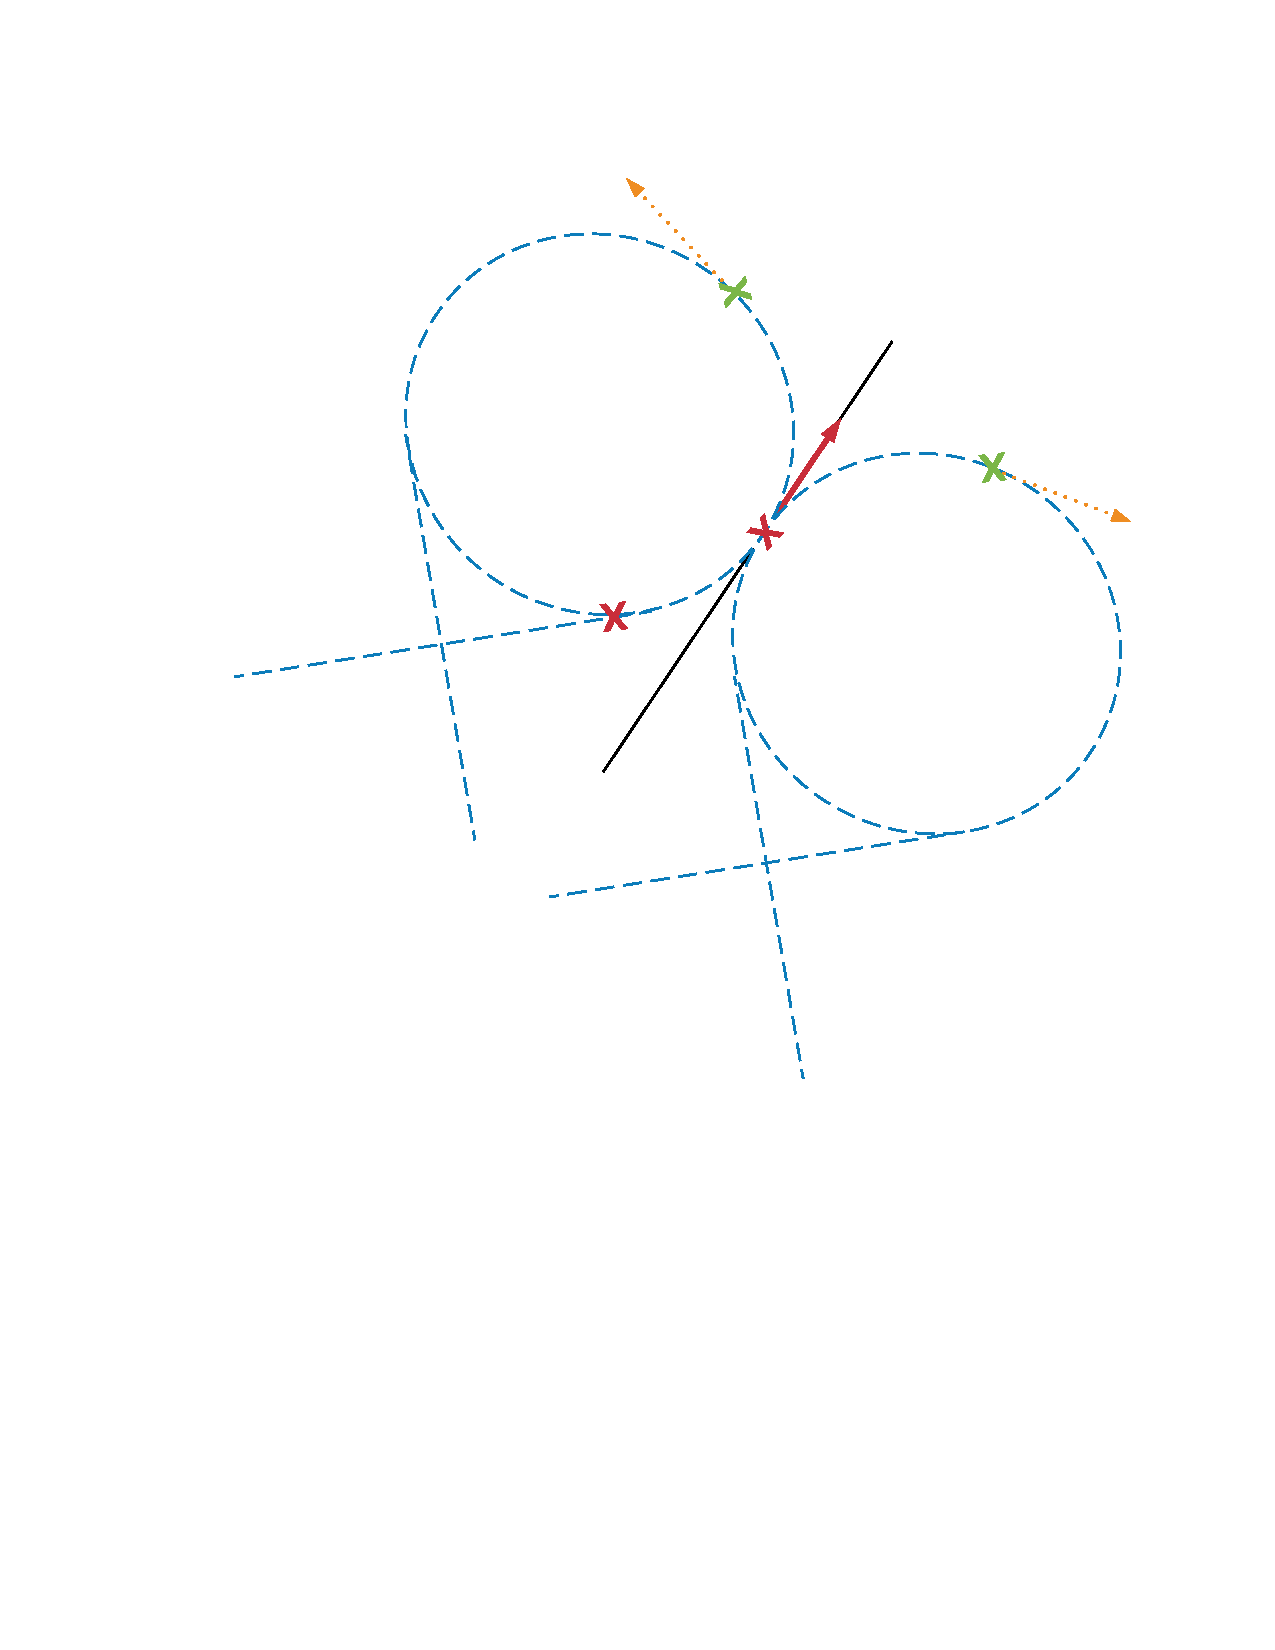
\includegraphics[width=\textwidth]{img/circular_movment6.pdf}
        \caption{Green crosses: future possible states of the platform at positions $(x_1^a,y_1^a)$ and $(x_1^b,y_1^b)$ .}
        \label{fig:six}
   \end{subfigure}
   
    \begin{subfigure}[b]{0.45\textwidth}
        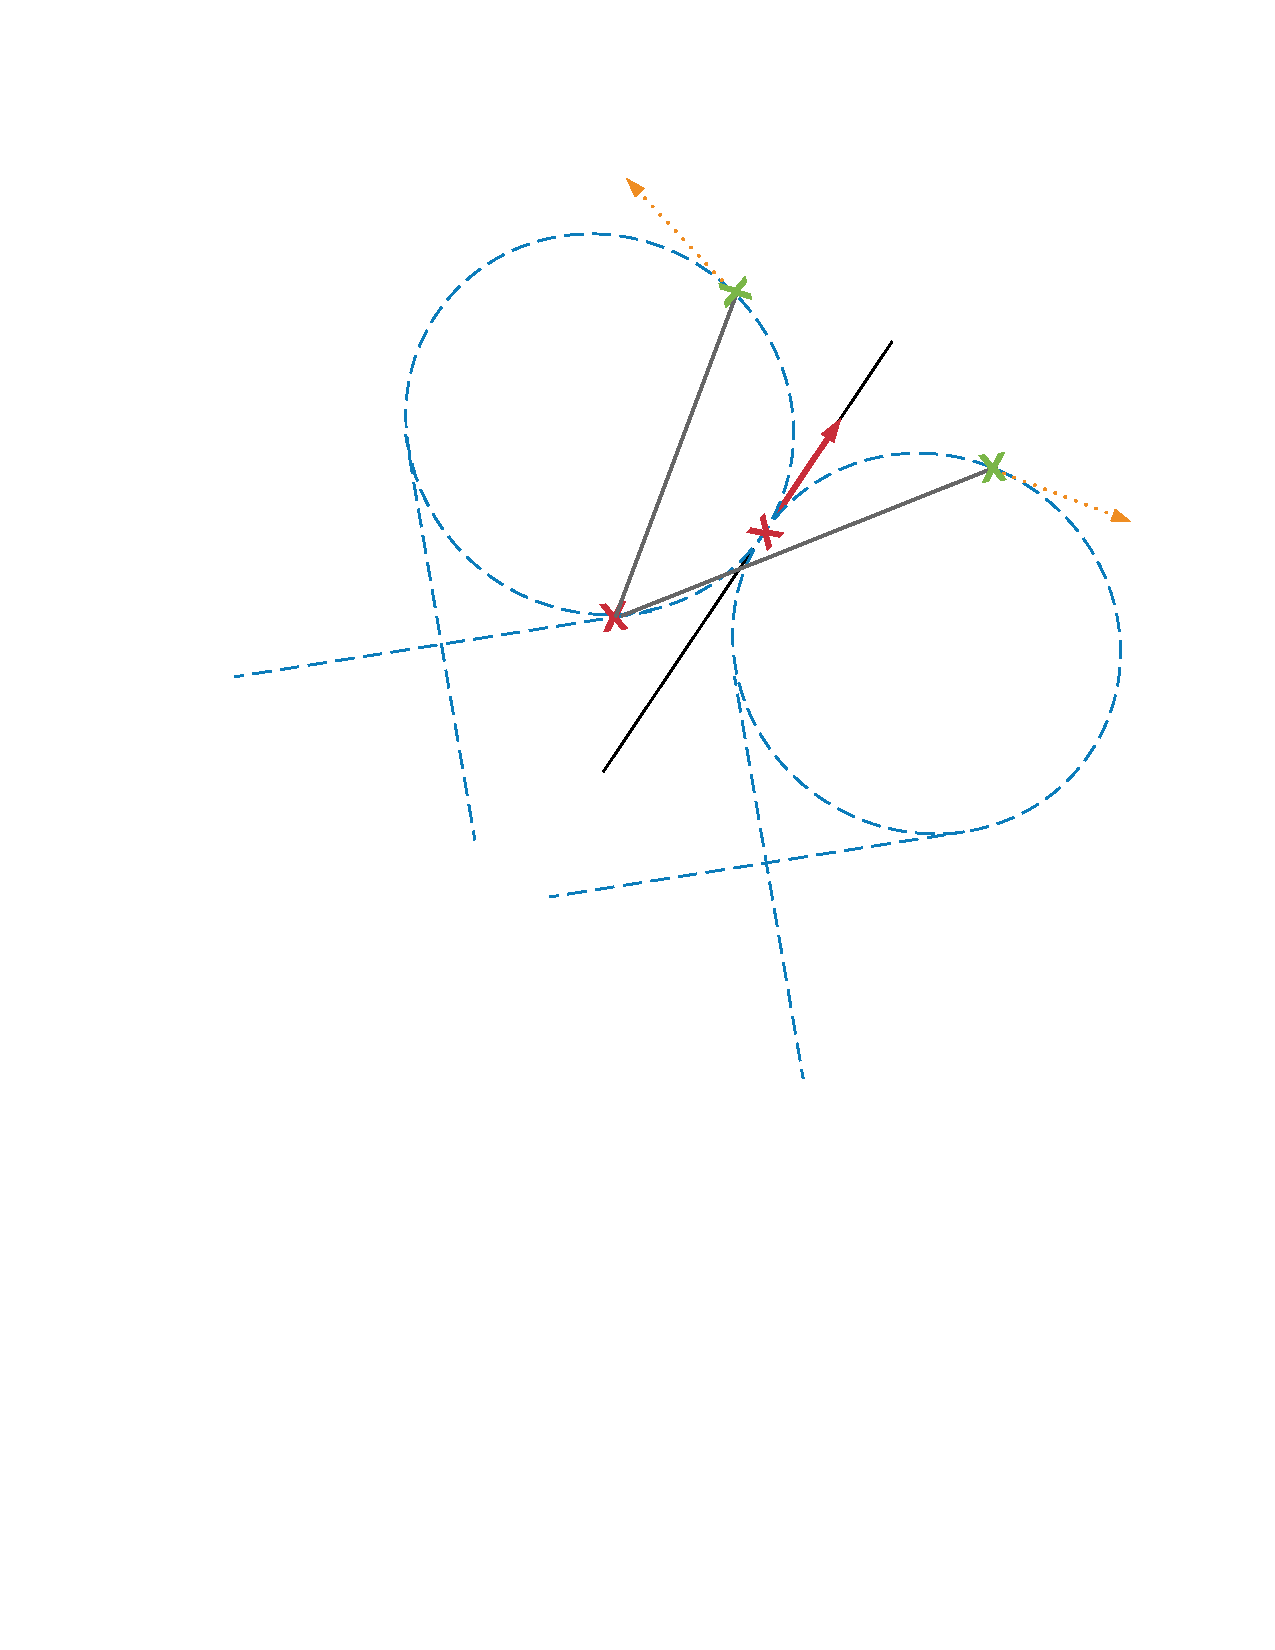
\includegraphics[width=\textwidth]{img/circular_movment7.pdf}
        \caption{Dark grey lines: distances from previous position at $t_{-\alpha}$ and possible future positions at $t_1$. }
        \label{fig:seven}
   \end{subfigure}\hfill
    \begin{subfigure}[b]{0.45\textwidth}
        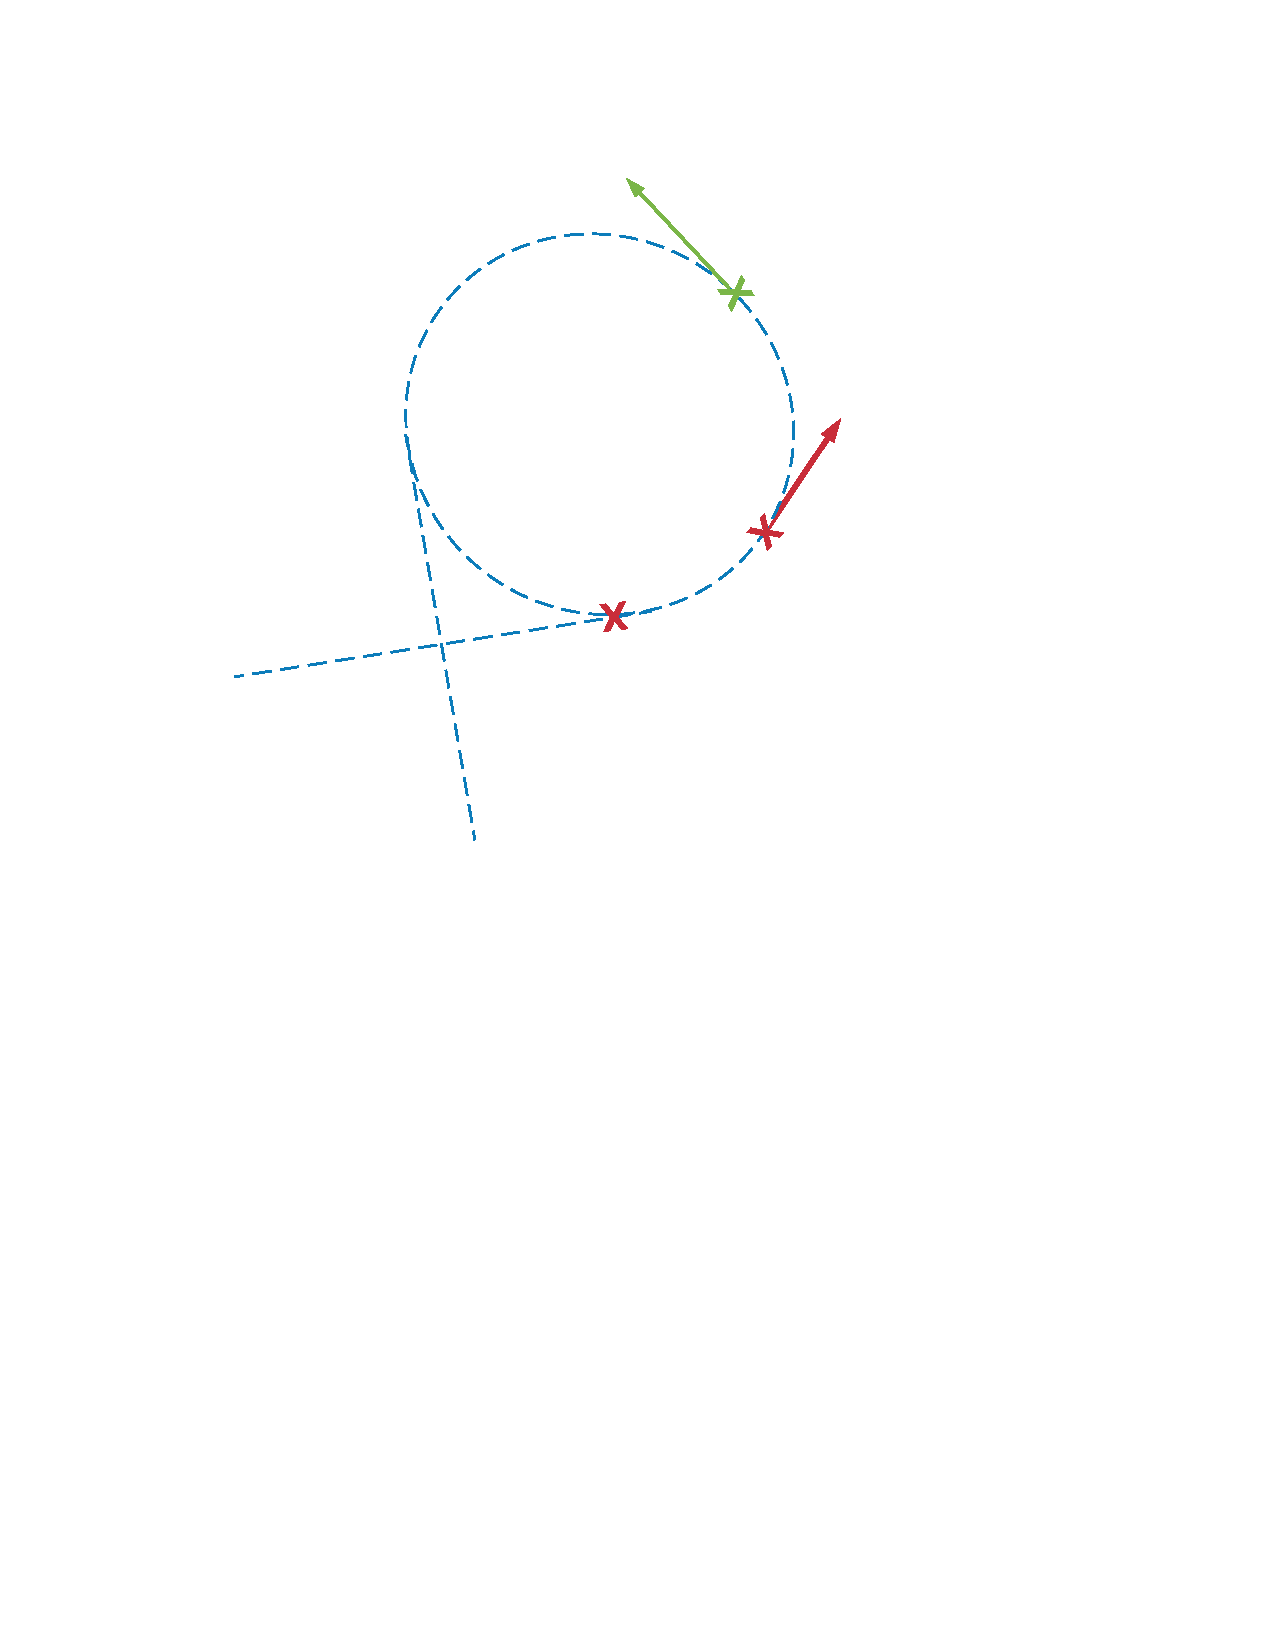
\includegraphics[width=\textwidth]{img/circular_movment8.pdf}
        \caption{Green cross with arrow: future state selected taking the position with minimum distance.}
        \label{fig:eight}
   \end{subfigure}
  \caption{The sequence of passages computed in order to select the future position when the platform is moving on the circumference.}
  \label{fig:sequence_find_next_position_circumference}
\end{figure} 
\end{itemize}

\newpage 
At this point we can use the predict position of the platform to control the quadrotor following the base.\\

The image \ref{fig:map_waypoints} shows the points in which the algorithm calculates where the quadrotor should go in order to following the moving car. It is noticeable the subdivision of point calculates with the linear model (green stars) and with the circular one (red stars).
% and also that the algorithm needs some time, $t_{curve}$, to understand the switch of movement regime and this can be seen in the delay in changing between calculation models.

\begin{figure}[!htbp]
    \centering
    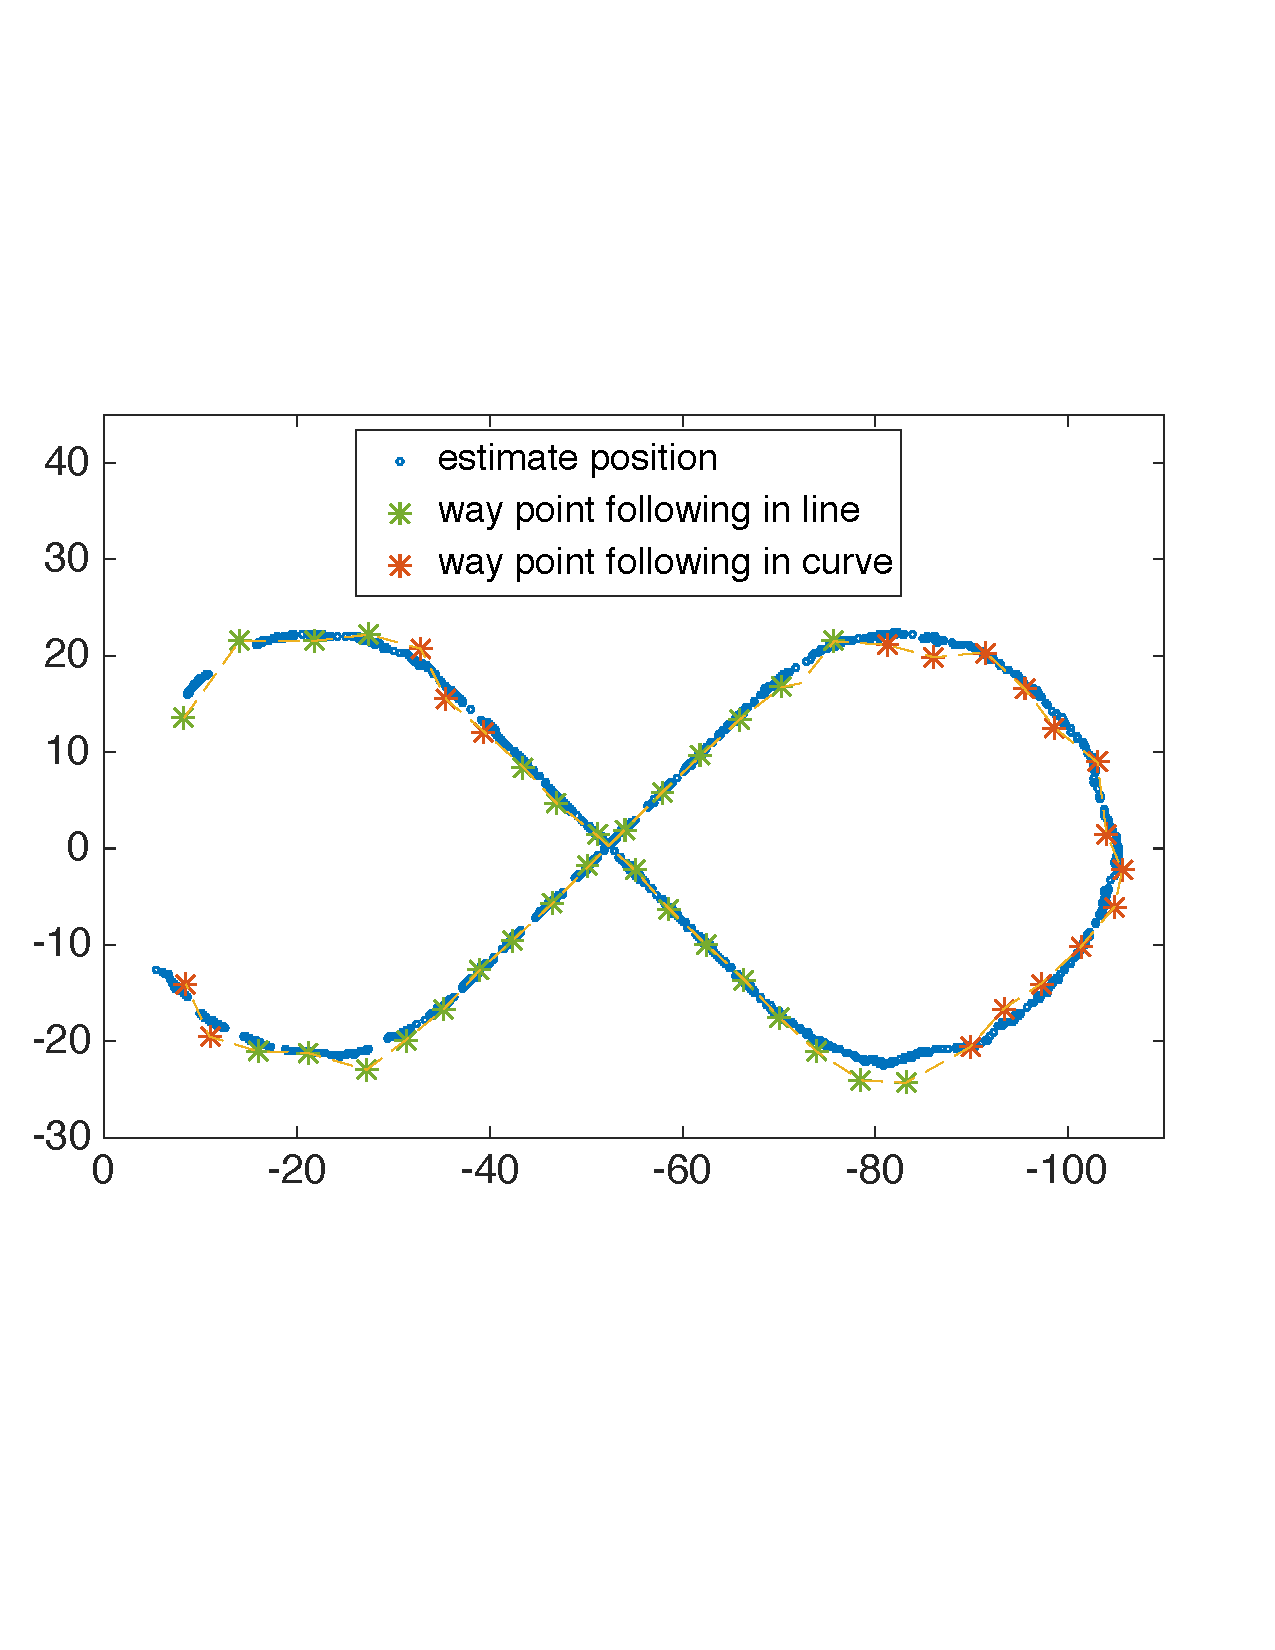
\includegraphics[width=0.8\textwidth]{img/following_platform_long_map_waypoints.pdf}
    \caption{Map of the estimated positions of the platform in blue.  Stars positions in which the quadrotor should go to following the base until a proper moment to proceed with the following stage is detected. The green points are calculated with the linear model while the red ones with the circular. }
    \label{fig:map_waypoints}
\end{figure}

\subsection{Select moment to land}
At this point the quadrotor is following the base, we have now to understand when the right moment to proceed with the other stages is arrived.\\
The right moment to start the landing maneuver is at the start of a line segment:
\begin{itemize}
\item if we detect the base and we understand that it is moving in the circumference we cannot land, we have to follow the base and waiting when we will detect a change in the regime from curve to line, at this point we can proceed with the following stages.\\
Proceed with the landing at this point can be risky if the platform is moving fast: as a matter of facts we know that the length of the straight line is $2\rho_8$ but we understand that the platform is moving straight after $l_{curve} = \frac{pi}{4}$ after it finished the curve, so the quad has just 
\begin{align*}
t_{landing} = \frac{\rho_8(2-\frac{pi}{4})}{v_{tan}}
\end{align*}
seconds to perform the land with the platform moving in line. If the velocity of the platform is too high this time could not be sufficient.
\item if we first detect the base and we understand that it is moving in a straight line we should not land, because we do not know when it actually started the line, so it can be almost at the end of it, and we do not have time to perform the entire landing maneuver.\\
What we do is following the car and waiting when it changes movement regime, from line to curve. At this point we can calculate where the next change point, from curve to line, will be and starting the landing at that point.\\
In this case we will have more time to complete the landing, because the quadrotor starts the maneuver at the begin of the line, no after $l_{curve}$, and, indeed, it can proceed with the first stage of the the landing even a little before the start of the segment, so:
\begin{align*}
t_{landing} \geq \frac{2\rho_8}{v_{tan}}
\end{align*}

In order to calculate where the future changing point will be, we must perform some computations:
\begin{itemize}
\item we know the orientation $\theta_{line}$ of the straight line just finished: the platform just changed from line regime to curve and we have saved the inclination $m$ of the best linear approximation found while it was moving in line.
\item given the point of change between line and curve, the future point will be in the circumference after an angle of $\big | \frac{3\pi}{2} \big |$.
\item from equations \ref{eq:anglechord} \ref{eq:lengthchord} we know that the segment connecting the change point and the future intersection point has length $\sqrt{2}\rho_8$ and angle $\theta_{line} \pm \frac{3\pi}{4} $
\item we can apply the same method described before to find the two possible intersection points:
\begin{align*}
\begin{cases}
x_{intersection}^a &= x_{changing} + \sqrt{2}\rho_8\cos{\Big(\theta_{line} + \frac{3\pi}{4}\Big) }\\[5pt]
y_{intersection}^a &= y_{changing} + \sqrt{2}\rho_8\sin{\Big(\theta_{line} + \frac{3\pi}{4}\Big) }\\[5pt]
\theta_{intersection}^a &=  \theta_{line} + \frac{3\pi}{2}
\end{cases}
\end{align*}
\begin{align*}
\begin{cases}
x_{intersection}^b &= x_{changing} + \sqrt{2}\rho_8\cos{\Big(\theta_{line} - \frac{3\pi}{4}\Big) }\\[5pt]
y_{intersection}^b &= y_{changing} + \sqrt{2}\rho_8\sin{\Big(\theta_{line} - \frac{3\pi}{4}\Big) }\\[5pt]
\theta_{intersection}^b &=  \theta_{line} - \frac{3\pi}{2}
\end{cases}
\end{align*}
and select the right one with minimum distance with the current estimate position of the platform.
\end{itemize}


The images  \ref{fig:sequence_find_next_intersection} summarize all the passages we perform to find the right intersection point just explained.

\begin{figure}[!htbp]
  \centering
   \begin{subfigure}[b]{0.45\textwidth}
        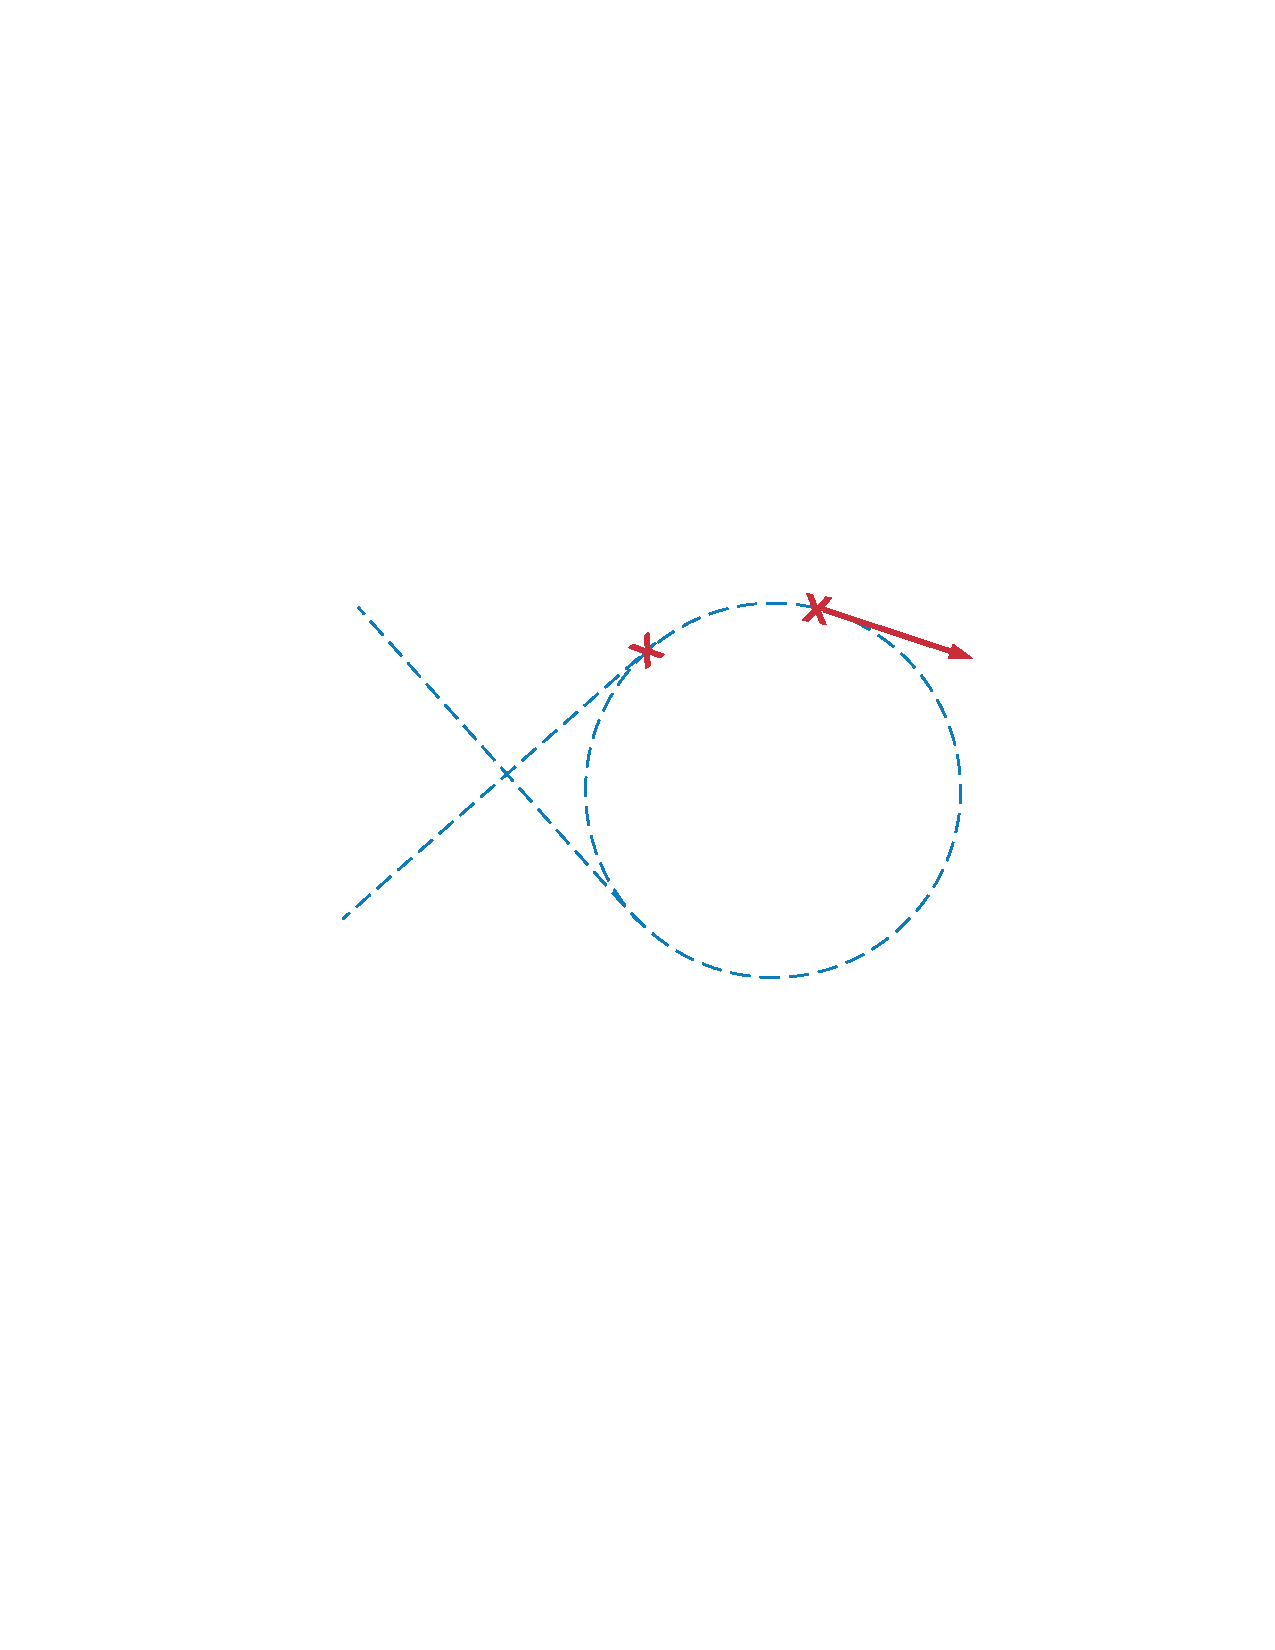
\includegraphics[width=\textwidth]{img/intersection_1.pdf}
        \caption{Red cross with arrow: state a $t_0$. Red arrow: current velocity vector. Red cross: changing point from line to curve.}
        \label{fig:one}
   \end{subfigure}\hfill
   \begin{subfigure}[b]{0.45\textwidth}
        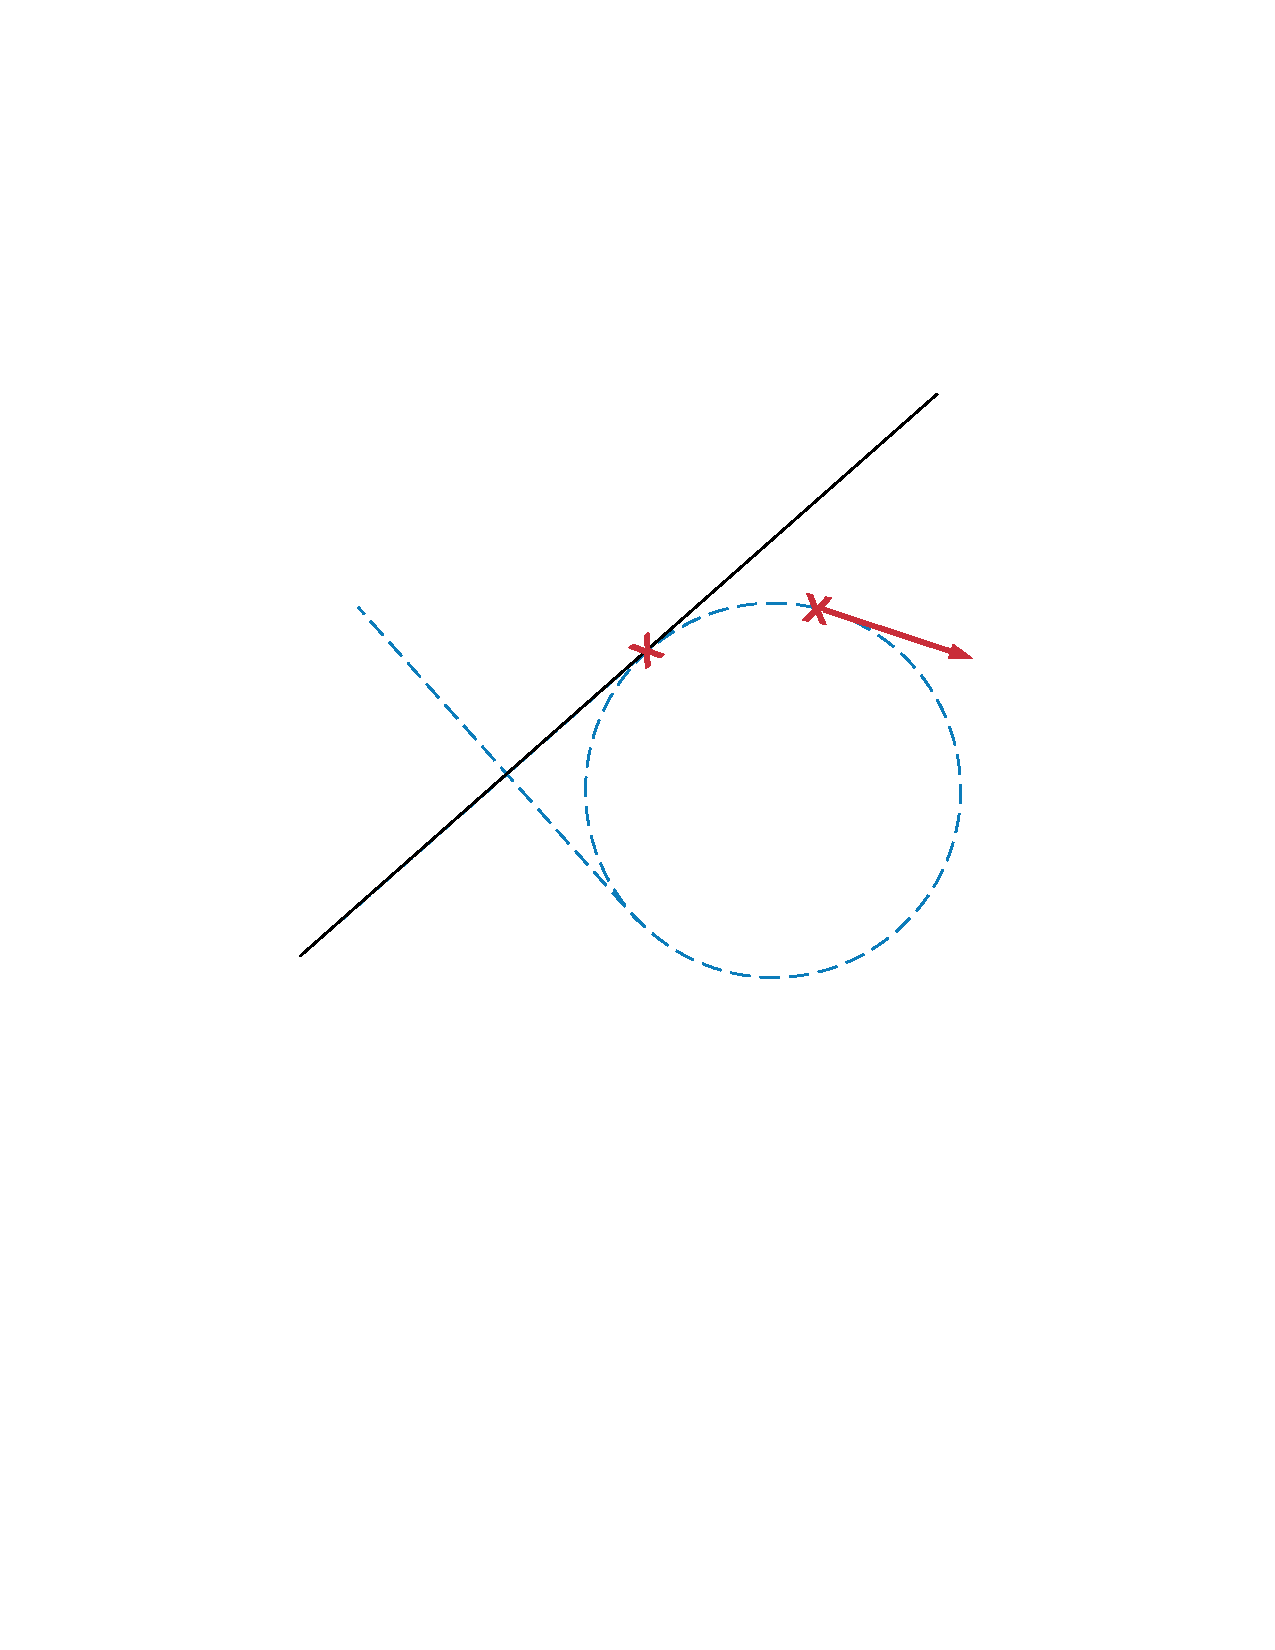
\includegraphics[width=\textwidth]{img/intersection_2.pdf}
        \caption{Black line: direction of the line sector just finished. The direction is taken as the slope of the best linear fit found in the previous regime.}
        \label{fig:two}
   \end{subfigure}
   
   \begin{subfigure}[b]{0.45\textwidth}
        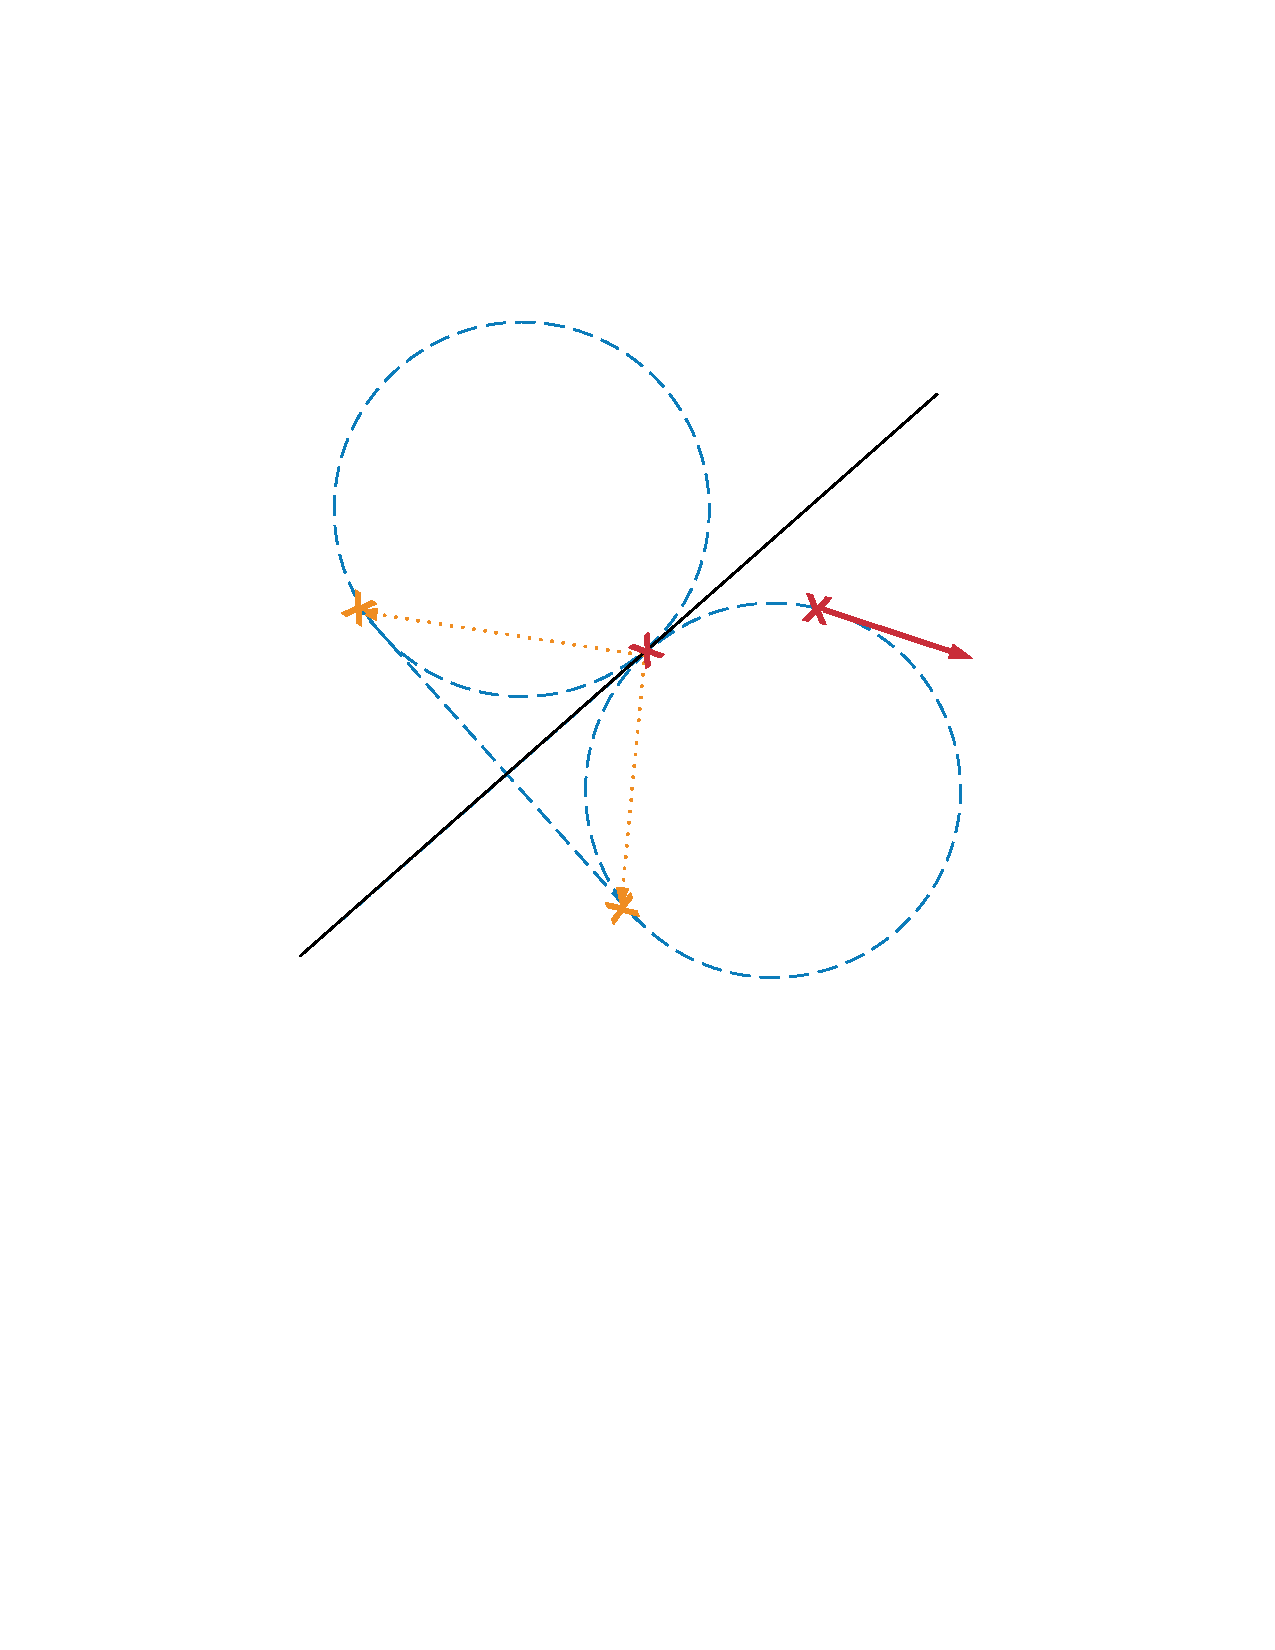
\includegraphics[width=\textwidth]{img/intersection_3.pdf}
        \caption{Blue lines: real and symmetric path. We do not know which of the two trajectories is correct. Yellow crosses: in both the path we can calculate the future intersection point.}
        \label{fig:three}
   \end{subfigure}\hfill
    \begin{subfigure}[b]{0.45\textwidth}
        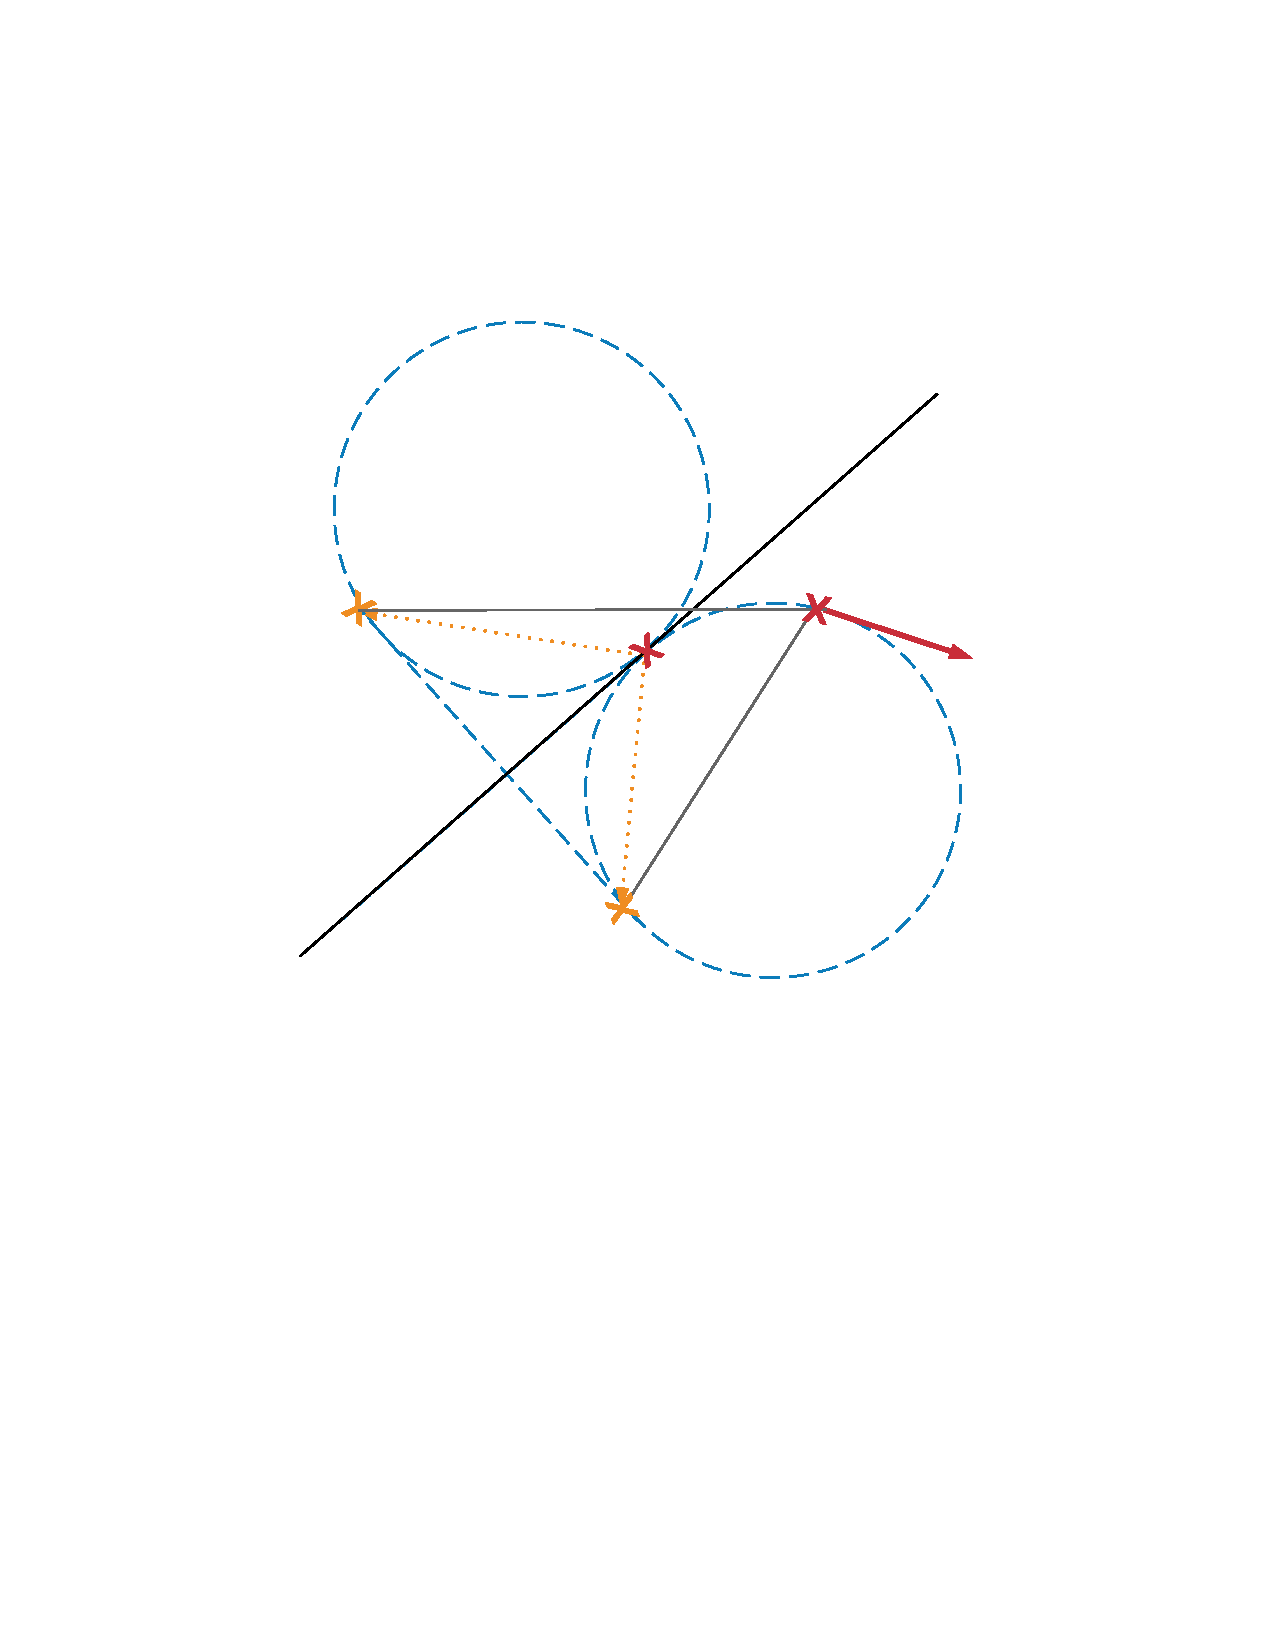
\includegraphics[width=\textwidth]{img/intersection_4.pdf}
        \caption{Dark grey lines: distances from current position and the two possible future intersections. Both are eligible becouse of the symmetry of the trajectory.}
        \label{fig:four}
   \end{subfigure}
   
    \begin{subfigure}[b]{0.45\textwidth}
        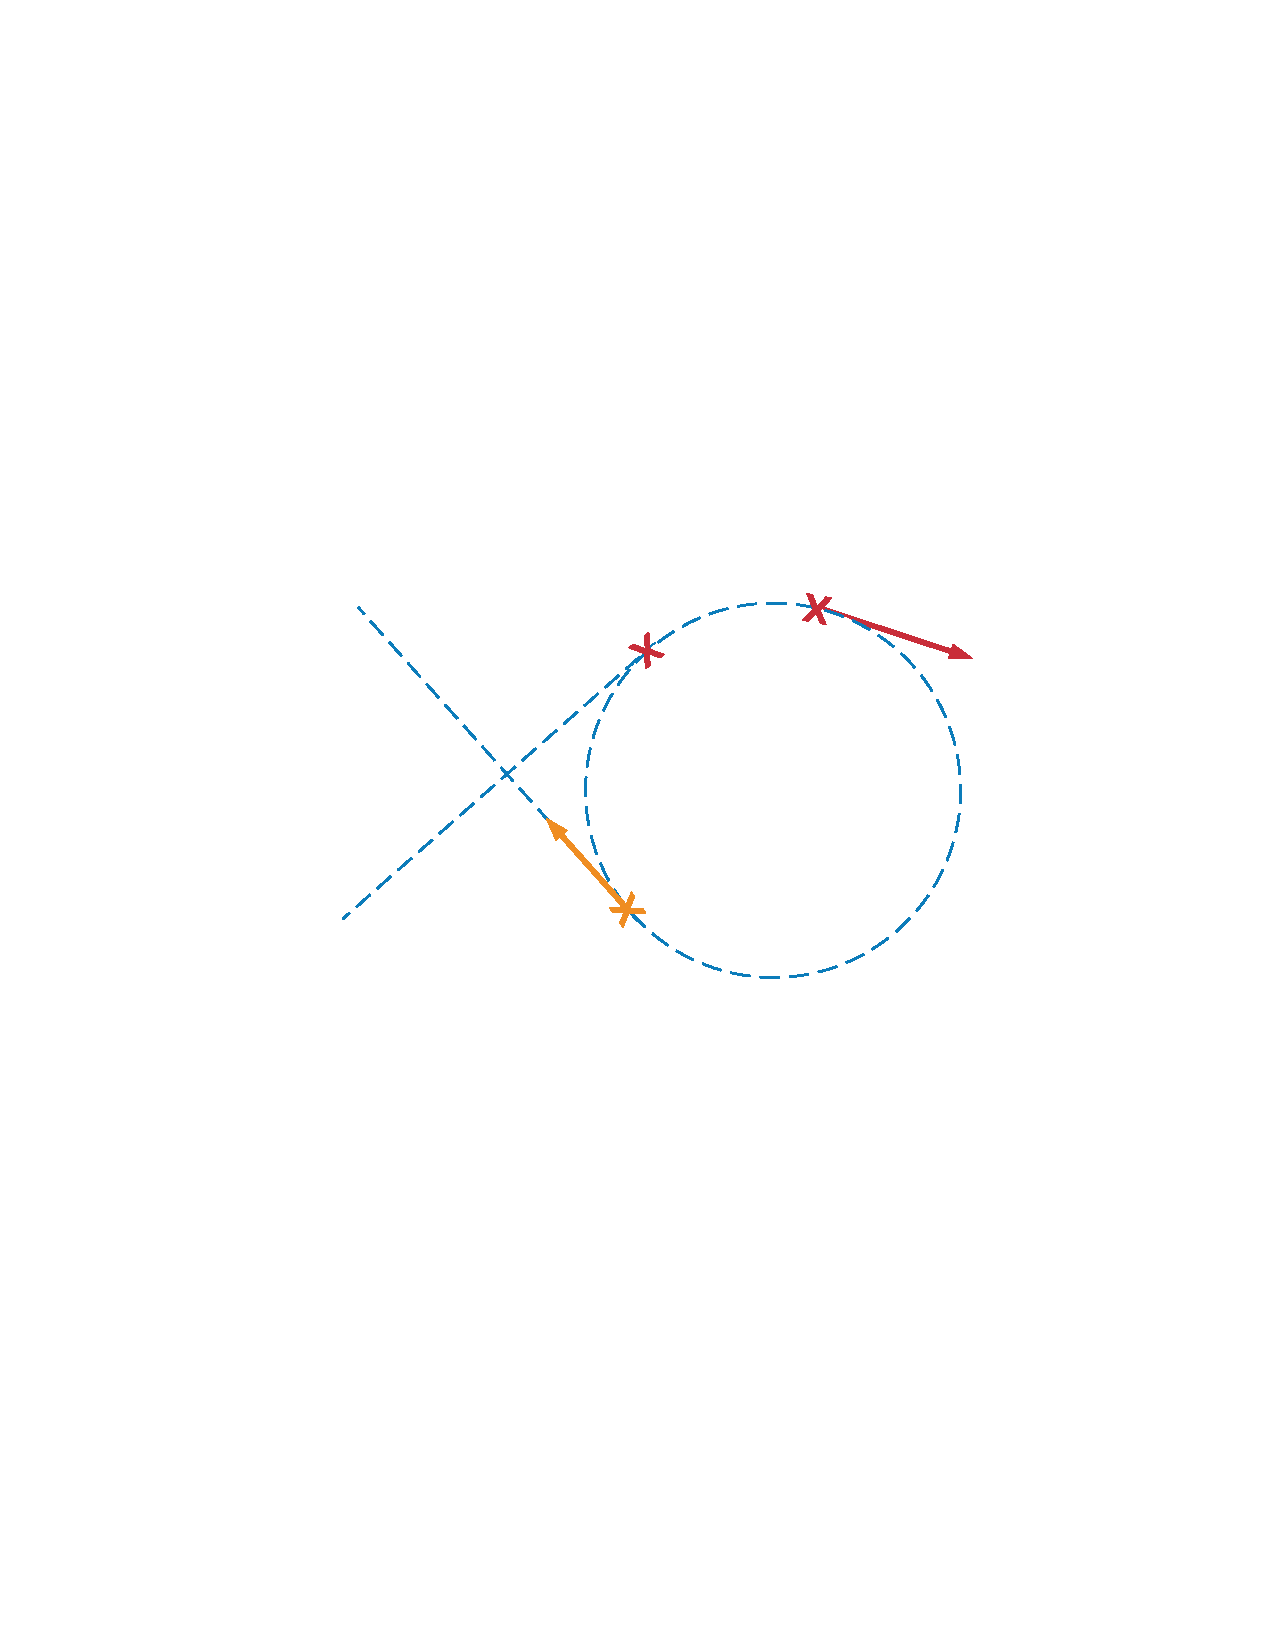
\includegraphics[width=\textwidth]{img/intersection_5.pdf}
        \caption{Yellow cross with arrow: future intersection point selected taking the position with minimum distance from the current state. }
        \label{fig:five}
   \end{subfigure}
  \caption{The sequence of passages computed in order to select the future intersection point where the platform will start the movement in line.}
  \label{fig:sequence_find_next_intersection}
\end{figure} 
\end{itemize}

\newpage
At this point the quad is keeping following the moving platform, but as soon as the base is near the future changing point, the quad can proceed with the next stage.\\

The image \ref{fig:map_intersections} shows where the algorithm calculates the future changing points (yellow crosses), based on the current one (red crosses). When the platform is in a neighborhood of these points for the UAV is the right moment to approach the base.

\begin{figure}[!htbp]
    \centering
    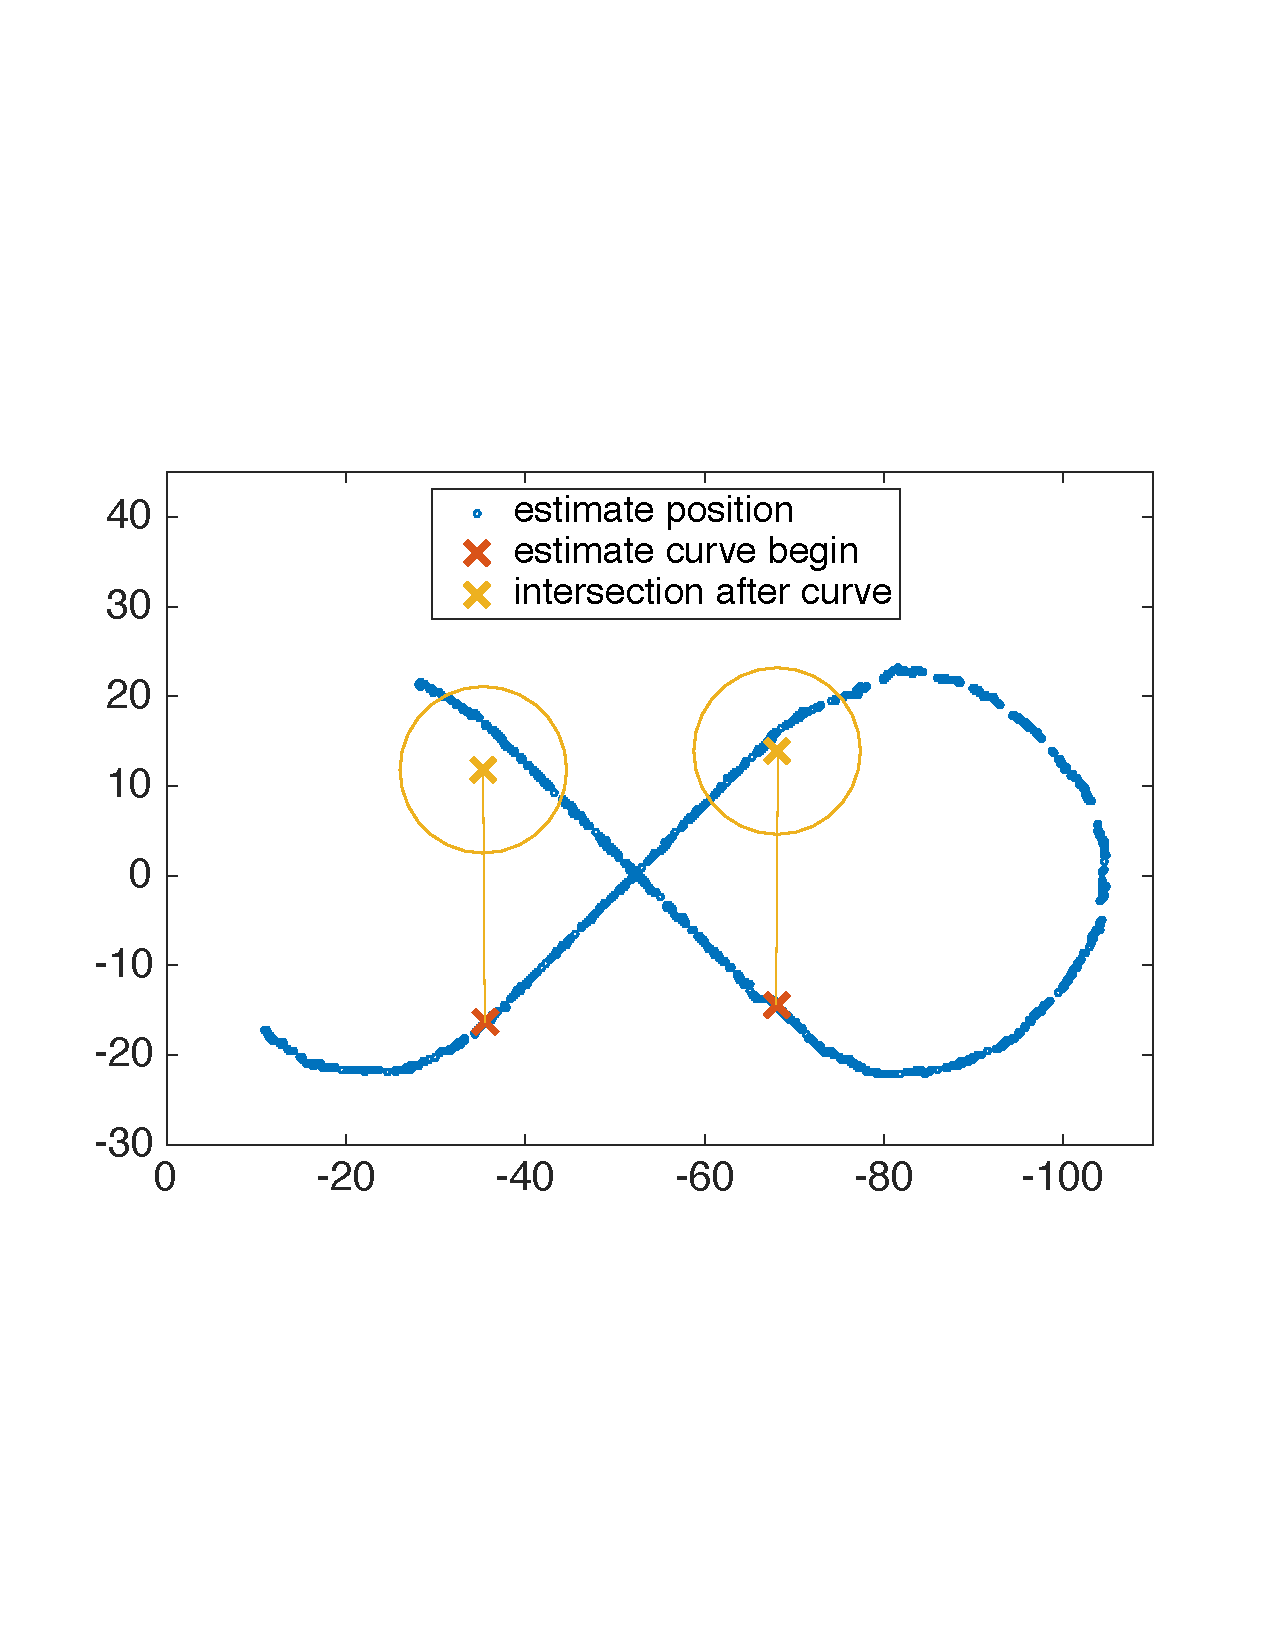
\includegraphics[width=0.8\textwidth]{img/following_platform_normal_map_intersection.pdf}
    \caption{Map of the estimated positions of the platform in blue.  Yellow crosses the position where the quadrotor should go in order to intersect the platform when is about to start a line phase.}
    \label{fig:map_intersections}
\end{figure}

\section{Approaching the base}
In this stage the quadrotor has to decrease its altitude keeping the platform in the fov until a better state estimation (from the low altitude EKF) is available.\\

The quadrotor is following the base and at high altitude. As soon as the platform start a straight line sector, the UAV must approach the platform reducing its altitude and keeping the target in the fov of the camera.\\
In this phase the desired final $x,y$ coordinates of the quadrotor are calculate with the same equations of the previous stage when a line movement of the platform is detected \ref{eq:line_future_pose}. 
The main difference are about the $z$ coordinate and the $x,y$ final velocities that the quad has to assume.\\
We set the final velocity identical to estimate velocity of the base:
\begin{align}
\begin{cases}
vx_1 &= v_{tan}\cos{\theta_0}\\[5pt]
vy_1 &= v_{tan}\sin{\theta_0}
\label{eq:finalstavelocity}
\end{cases}
\end{align}
While the final altitude:
\begin{align}
z_1 = \alpha z_0 + (1 - \alpha) z_{0,target}
\label{eq:finalz}
\end{align}
Where $\alpha <  1$ is a parameter to be tuned in order to have a right balance between fastness of this stage and aggressiveness of the maneuver.\\
As a matter of fact if the quad approaches too quickly the target, it is very easy to lose the platform from the fov of the camera: the closer we are to the base the less area we can cover with the camera, so the more precise we must be in order to still have tracking of the target.\\

If we set the final state of the quad with the state estimation of the moving base we have from high altitude ($\alpha = 0$) 
we are directly performing the landing on the base, but the UAV could approach a final position that is not the right one and so it can loose the platform. It is necessary to have some intermediate stages in which the quad is getting closer to the platform, so it can refines and correct the final target, but the area spanned by the camera is large enough to detect the base even if the quad is not in the right pose.\\
If we loose the platform, this stage fails, and we have to takeoff again until the platform is in the fov again.\\
The figure  \ref{fig:approach_platform} summarize a situation in which approaching the platform too aggressively can lead to the loss of tracking, while if we have intermediate steps we can recover from the estimation error we had.\\ 

With this approach the platform can stay in the fov of the camera much easier:  the quad is going ahead of the base, with a direction that is the same of the target, and correcting the estimate position of the moving platform at each step. \\
As soon as we are close enough to have a more precise state estimation from the low altitude EKF we proceed with the next stage.

\begin{figure}[!htbp]
 \centering
   \begin{subfigure}[b]{0.8\textwidth}
     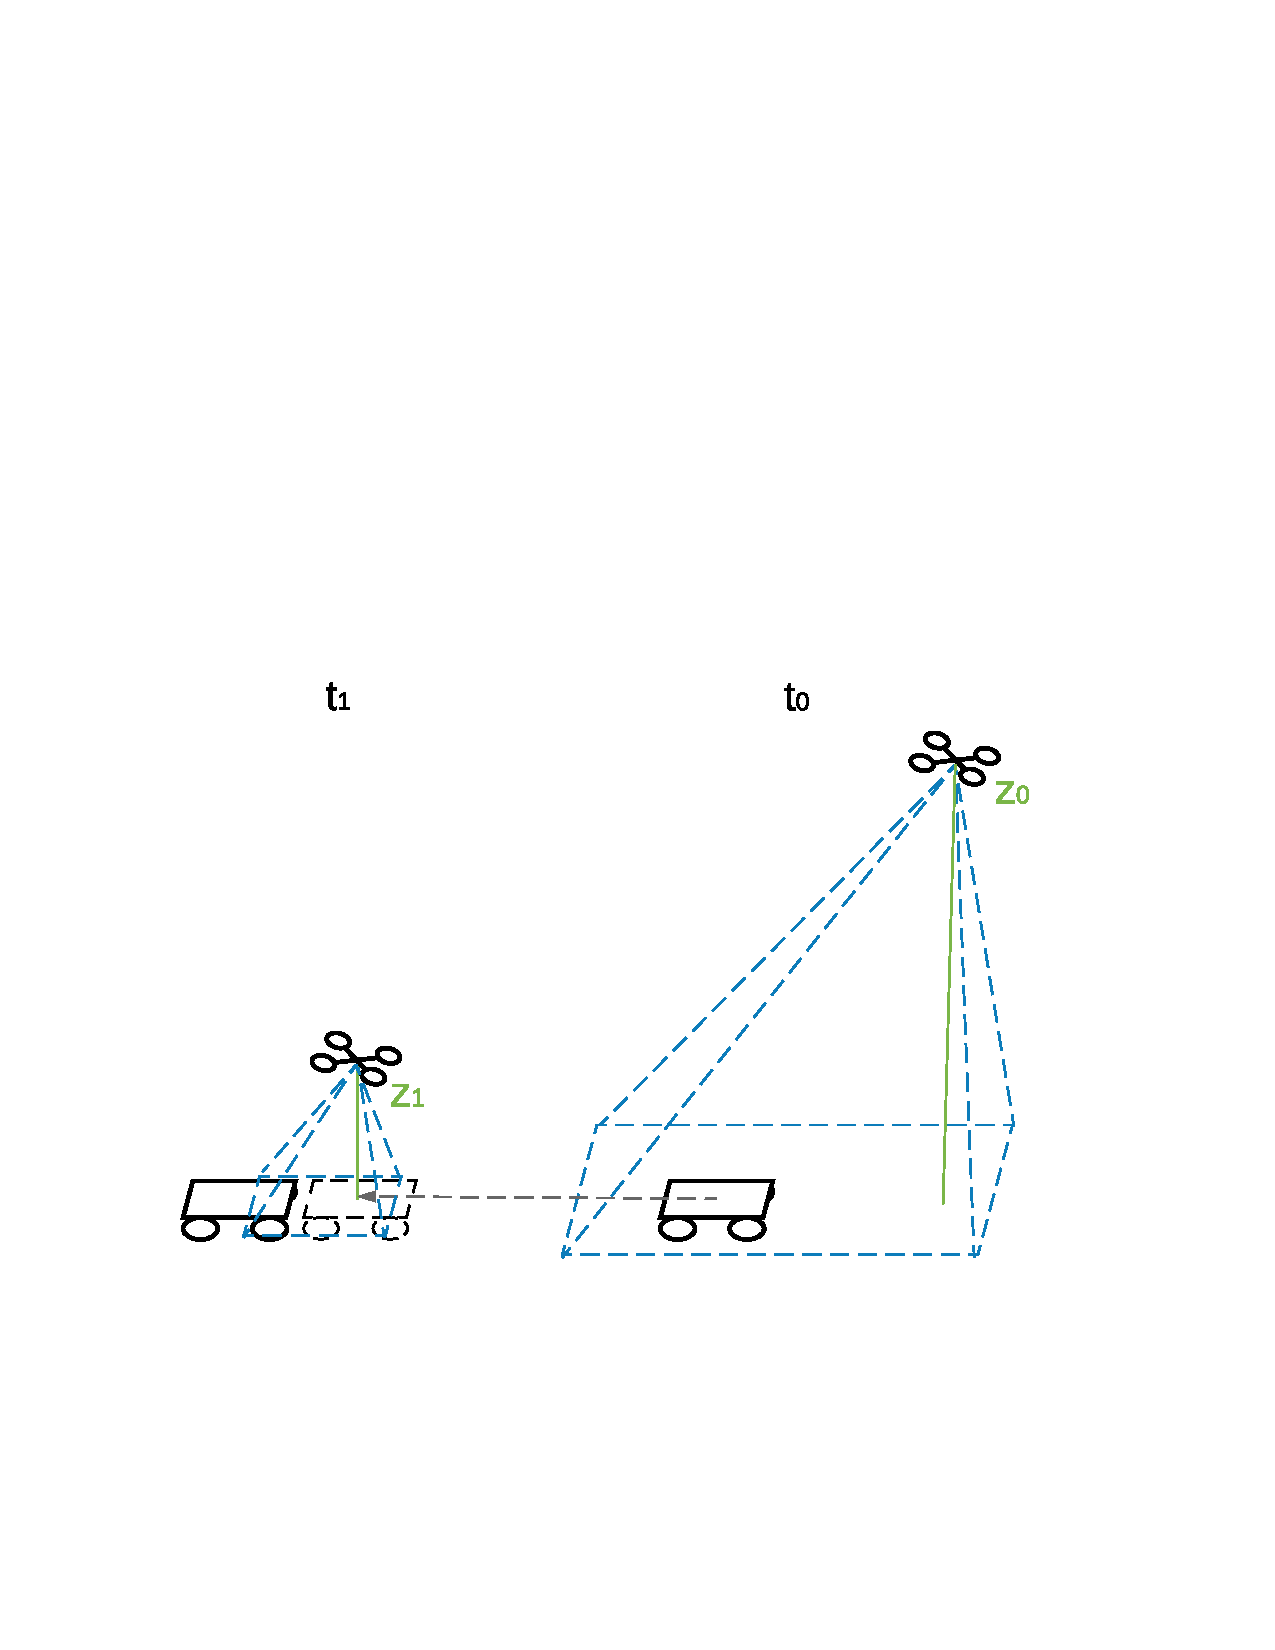
\includegraphics[width=\textwidth]{img/approach_platform_lose.pdf}
        \caption{If we set $z_1$ too close to the platform we can loose the tracking because the position estimation of the moving base is not good enough from high altitude.}
        \label{fig:loose_platform}
   \end{subfigure}
 \end{figure}
\begin{figure}[!htbp] \ContinuedFloat  
   \begin{subfigure}[b]{0.8\textwidth}
     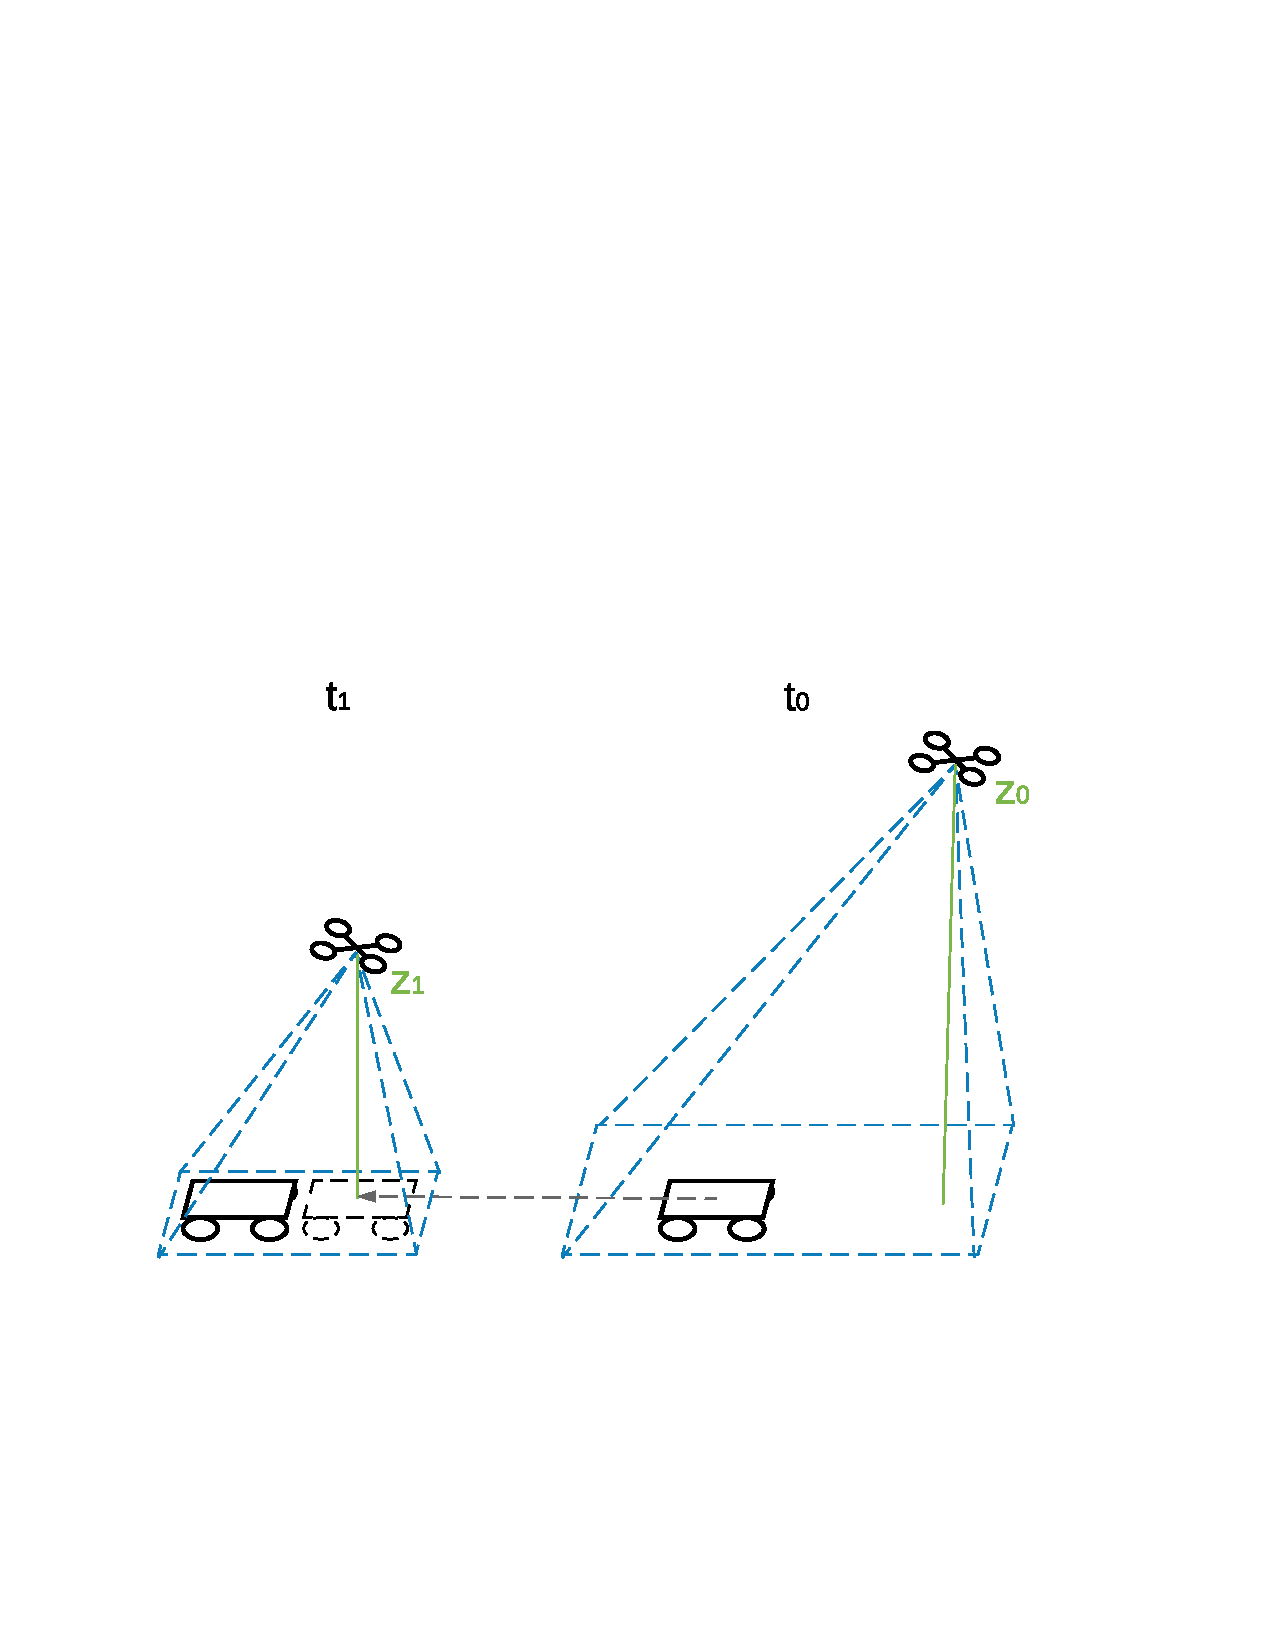
\includegraphics[width=\textwidth]{img/approach_platform.pdf}
        \caption{With intermediate steps, instead, it is more difficult to loose the platform and we can correct the state estimation.}
        \label{fig:not_loose_platform}
   \end{subfigure}
    \caption{The scheme describe a situation in which intermediate steps, while approaching he moving platform from high altitude, are necessary to not loose the platform.  }
    \label{fig:approach_platform}
\end{figure}
 
\section{Align with the base}
In this stage the quadrotor is flying close to the platform and before proceeding with the landing maneuver it has to align its direction with the base to be in the best position to proceed with the final step.\\

When a state estimation of the base from the low altitude EKF is available the quad can relay on this information
to align its movement with the base. The estimation is good enough to predict the future states of the moving platform even if we loose tracking. As a matter of fact in this stage we know that the platform is moving in a straight line, we now its initial position, direction and velocity, so it is easy to predict where it will be in $t$ seconds.\\

Given the current state of the platform and of the UAV we can calculate the distance $d$ between the two. This segment can be covered by the quadrotor with an maximum relative speed:
\begin{align}
v_{max,rel} &= v_{max,quad} - v_{base}
\label{eq:relative_vel}
\end{align}
In a time:
\begin{align}
t &= \frac{d}{||v_{max,rel}||}
\end{align}
We can see from equation \ref{eq:relative_vel} that if the maximum velocity of the quadrotor  is equal in magnitude and opposite direction with respect to the velocity of the platform the time $t$ to reach the platform is infinite.\\

In this period of time we know that the platform is moving to a different place, and we have to predict where it will be in $t$ seconds.\\
To predict the future position we are using the same model used in the EKF \ref{eq:equation_nonholonomic_discrete}. With this model we do not just predict where the platform will be after $t$ seconds, but we estimate its state for discrete moments in a window of time around $t$: $[t-t_1,t+t_2]$. In this way we have a set of possible future position that the quadrotor must be able to reach perfectly in time to intersect the platform.\\
It is also possible to bring the quad ahead of the platform simply requiring to reach a state of the window in less time.\\

This window of future state estimate is used by the trajectory generator module to calculate different possible alternatives to reach the platform.\\
In this stage the final target of the quadrotor will be one of these odometry estimations with $x,y$ position and velocity equal to the one of the platform, and $z$ position set to a proper height $h_{align}$.\\

\begin{figure}[!htbp]
    \centering
    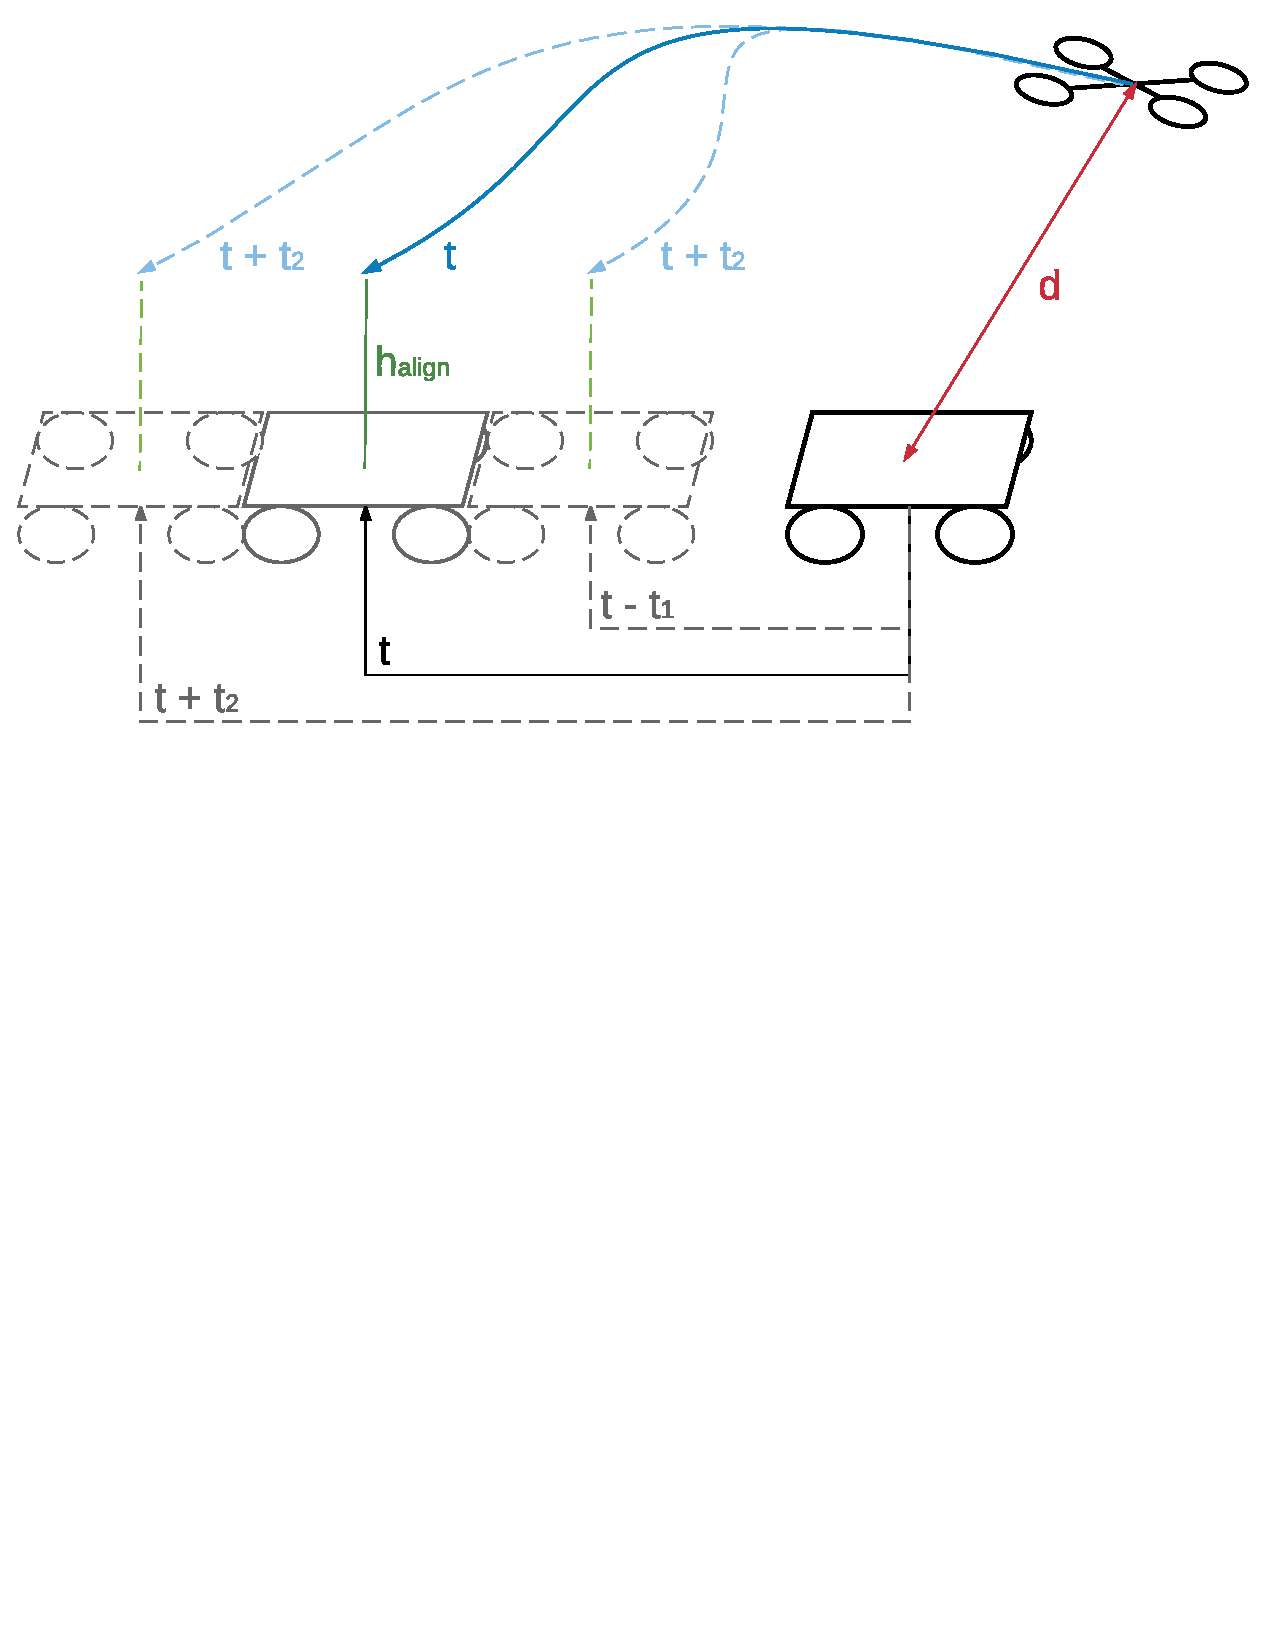
\includegraphics[width=0.8\textwidth]{img/prediction_platform.pdf}
    \caption{The scheme synthesizes the algorithm performed in this stage to find the possible final states in which the quadrotor should reach in order to intercept the base. }
    \label{fig:align_platform}
\end{figure}

As soon as the quadrotor reaches the final target state, in which it is align with the moving platform, and the final target was in the fov recently, we proceed with the final stage.

\section{Landing on the base}
In this final stage the quadrotor is very close to the platform and is moving in the same direction. It has to decreases its altitude until it touches the platform and then switches off the motors in order to conclude the whole task.\\

The way to calculate the final target is equal to the previous stage of the state machine: we predict possibles intersection points that can be reachable by the quadrotor, and the final states of the UAV will be one of these odometries.\\
It is possible also to add a velocity and/or acceleration in the $z$ direction in order to have a slightly more aggressive vertical landing.\\
Furthermore because the visual odometry can fails when we are really close to the platform we introduce the possibility of a blind landing, in which we are not using the state estimation of the quadrotor to control the UAV, but we control the thrust in an open loop: when we are at $h_{blind}$ over the platform we start to apply a thrust $c_{quad}$ such that $||c_{quad}|| < g$ in order to decrease the altitude of the quadrotor until it touches the platform.\\
In detail the quad in this phase is moving in the z axis with the following kinematics:
\begin{align}
\begin{split}
z(t) = z_{quad,0} + vz_{quad,0}t + \frac{(c_{quad,z} - g)t}{2}
\label{eq:z_dynamics}
\end{split}
\end{align}
If the quad starts from $z_{quad,0} = h_{blind}$ after a time $t_{blind}$ we want $z(t_{blind}) = 0$. furthermore we consider the initial velocity in $vz_{quad,0}$ really little, so it can be neglect. We can then easily calculate the time $t_{blind}$:
\begin{align}
\begin{split}
t_{blind} = \sqrt{\frac{2h_{blind}}{g-c_{quad,z}}}
\label{eq:z_dynamics}
\end{split}
\end{align}

We know that in this time $t_{blind}$ the platform will changed its position, in particular it is moving in a straight line, so its coordinates will be :
\begin{align}
\begin{cases}
x_{base}(t_{blind}) &= x_{base}(0) + v_{tan}t_{blind}\cos{(\theta_{base})}\\[5pt]
y_{base}(t_{blind}) &= y_{base}(0) + v_{tan}t_{blind}\sin{(\theta_{base})}
\end{cases}
\label{eq:future_pose_blind}
\end{align}

So we know that if we have selected the coordinates $\tilde{x},\tilde{y}$ as intersection points where we will start the blind landing over the platform, the quad must be at these coordinates $t_{blind}$ seconds before the platform in order to properly land over it (notice that if $h_{blind} \rightarrow 0$ also $t_{blind} \rightarrow 0$ and so the quad arrives at the intersection point with the moving base).\\

\begin{figure}[!htbp]
    \centering
    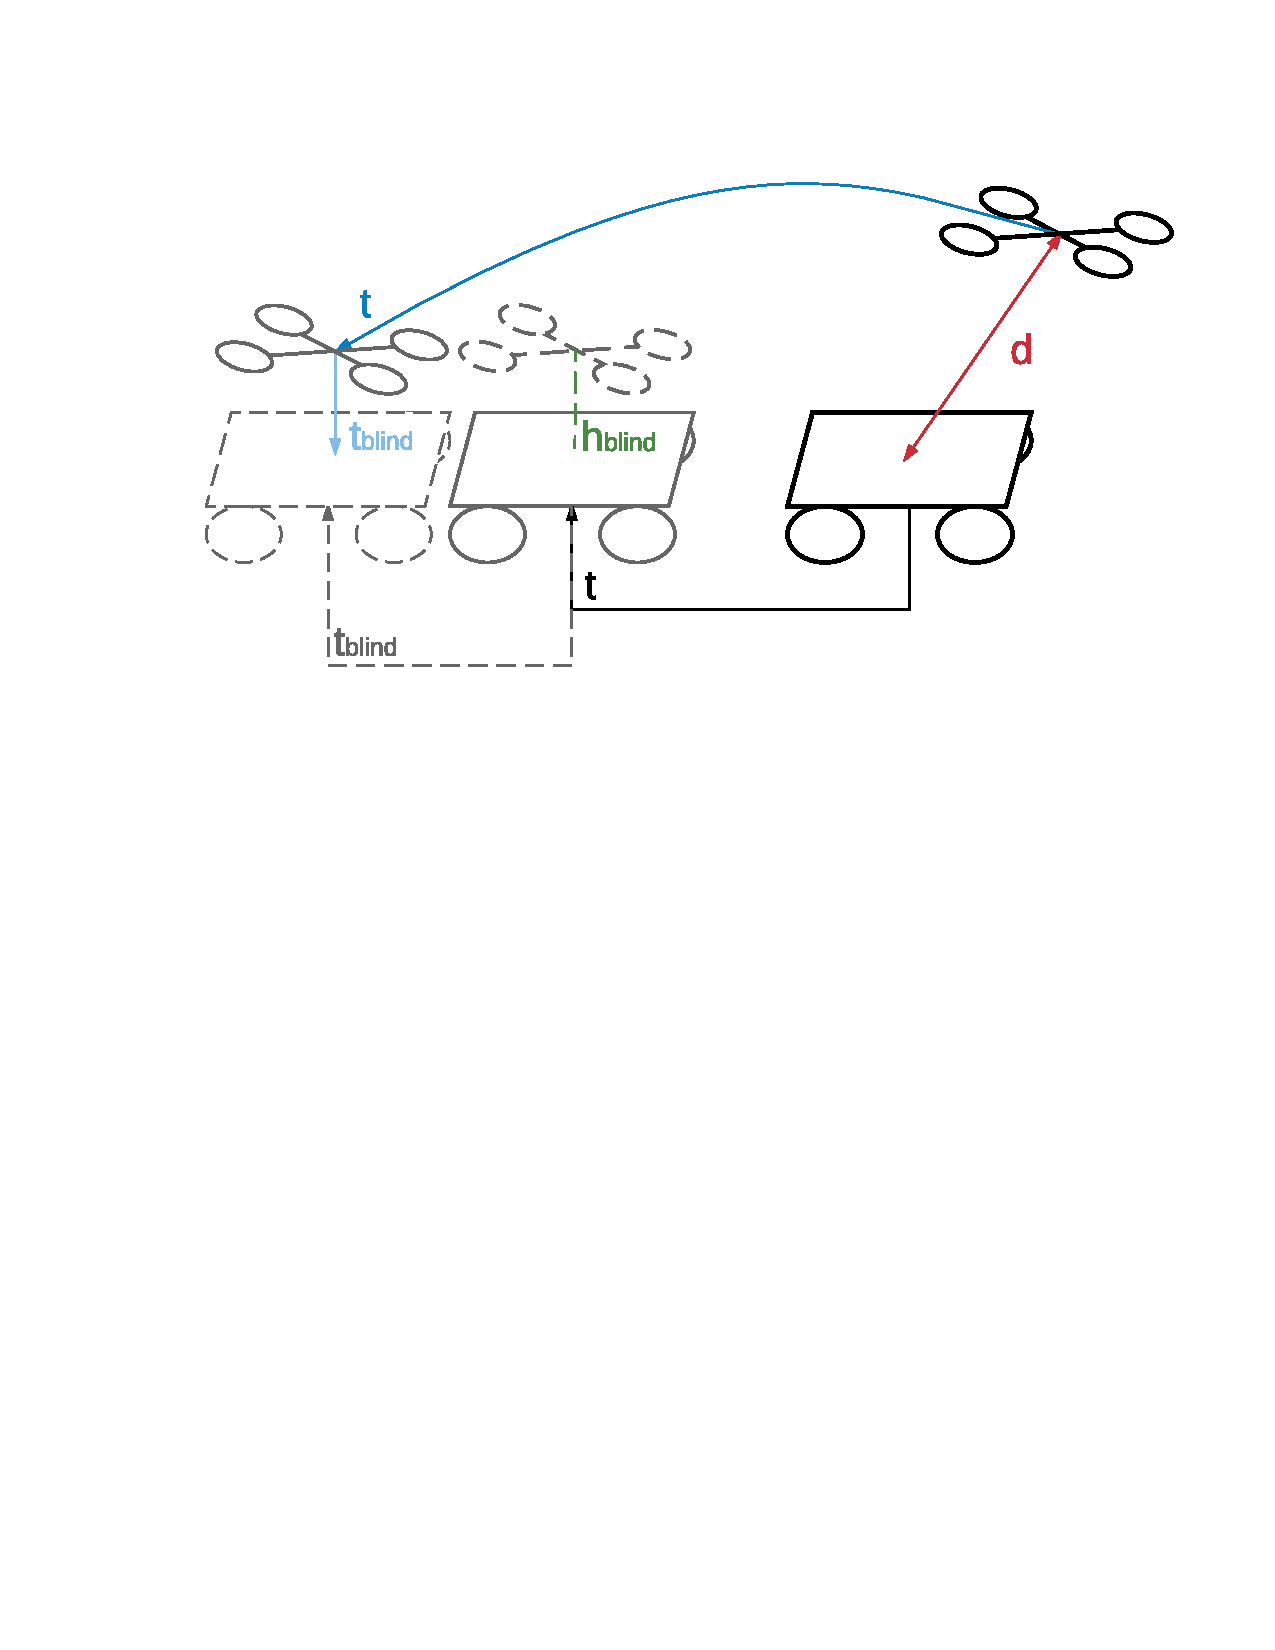
\includegraphics[width=0.8\textwidth]{img/blind_landing.pdf}
    \caption{The scheme synthesizes the concept of the final blind landing. }
    \label{fig:align_platform}
\end{figure}

In order to detect when the quad is touching the platform we check the data from the IMU. \\
This unit is given different measurements, among which the value of the linear accelerations along the 3 axes. Using this data we can calculate the magnitude of the acceleration and we know that when the UAV is hitting a surface this quantity is showing a big pick, so with a simple threshold on the acceleration norm we can detect when the quadrotor is landed.\\
This solution does not take in account that data from the IMU are usually corrupted by noise (see \ref{subsec:acceleration}) and so we could confuse a noisy measurement with a bump. \\
To make this detection more robust we can filter the data with a low pass filter:
\begin{align}
imu_{filt}(t_k) =  (1-e^{-\frac{t_k-t_{k-1}}{\tau_{imu}}})imu_{raw}(t_k) + e^{-\frac{t_k-t_{k-1}}{\tau_{imu}}} imu_{filt}(t_{k-1})
\label{eq:imu_filtered}
\end{align} 
The filter eliminates the noise but it slows down the response to changes, so the detection of the bump is done with some delay: the parameter $\tau_{imu}$ is deciding the cut frequency of the filter, so tuning this quantity can lead to a final filtered data with the right balance between smoothness and sensibility to changes.\\  

These methods that uses the absolute value of the acceleration, do not take in consideration that the quadrotor could assume a very high acceleration while is performing a normal flight, and so this acceleration could exceed the threshold and be detected as a bump.\\
Another solution to have a robust and fast bump detector is to compare the raw data from the IMU with the filtered one: only the bump creates a big change that the filter cannot follow instantaneously, so the difference between the two version of the data will be very high only in this occasion.\\
The figure \ref{fig:imu_landing} shows the data used by the bump detector in order to find when the quad is touching the platform and switch off the motors.

\begin{figure}[!htbp]
    \centering
    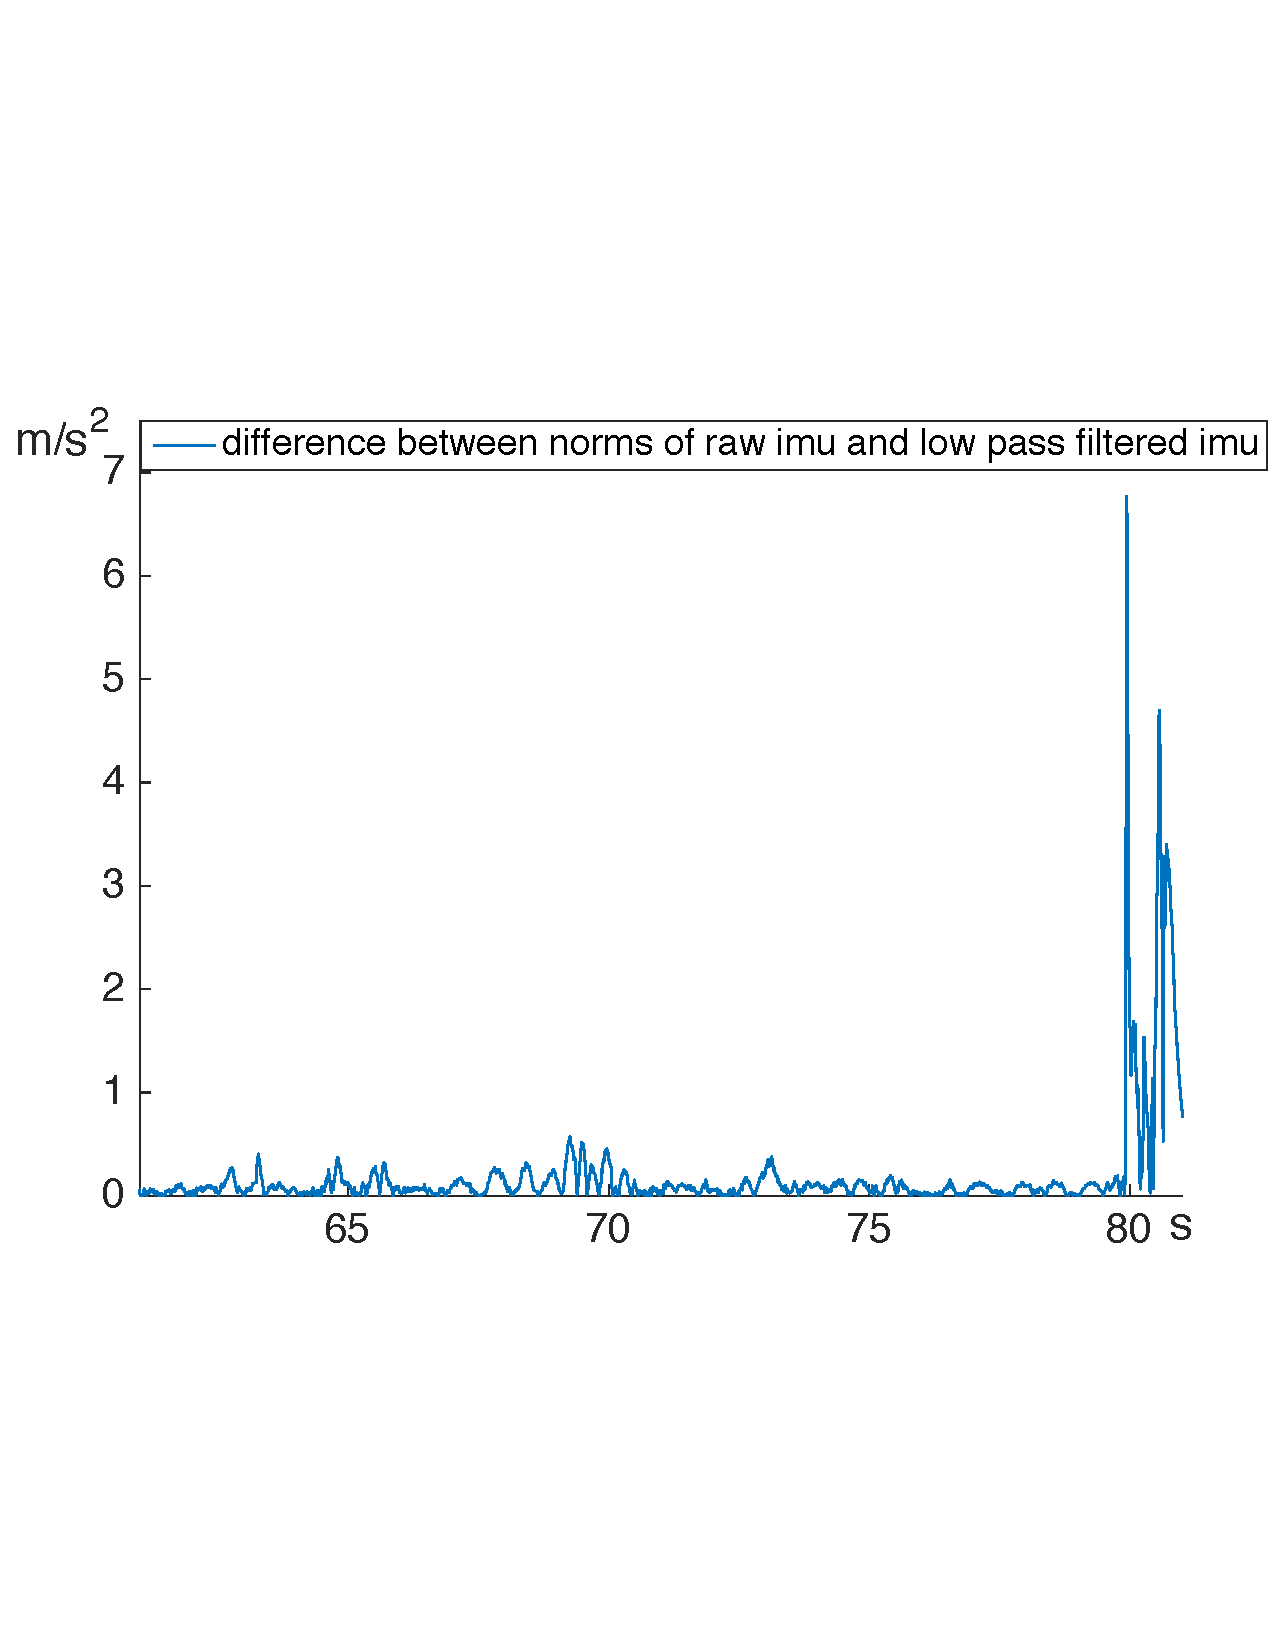
\includegraphics[width=0.72\textwidth]{img/imu_landing.pdf}
    \caption{Data used by the bump detector: difference between the norms of the raw data from the imu and the filtered version of the same. The difference is growing really fast only when the UAV bumps on the surface.}
    \label{fig:imu_landing}
\end{figure}
 
If something goes wrong and in this phase the quadrotor reaches a $z_{quad} < z_{base}$, then the landing failed and we have to takeoff again.
